% =============================================================================
%  Two-Stage Calibration of Decomposable Web Ranking
%  English manuscript.  Compile with:  xelatex paper_en && xelatex paper_en
%  Every number in the text comes from generated/macros.tex and every table from
%  generated/en/, both written by ../make_paper_assets.py from the saved results.
% =============================================================================
\documentclass[11pt,a4paper]{article}
\usepackage[a4paper,margin=2.3cm]{geometry}
\usepackage{amsmath,amssymb,amsthm}
\usepackage{txfonts}
\usepackage[no-math]{fontspec}
\setmainfont{FreeSerif}
\setmonofont{DejaVu Sans Mono}[Scale=0.82]
\usepackage[english]{babel}
\usepackage{graphicx}
\usepackage{booktabs}
\usepackage{array}
\usepackage[font=small,labelfont=bf]{caption}
\usepackage{enumitem}
\usepackage{algorithm}
\usepackage{algpseudocode}
\usepackage{microtype}
\usepackage{placeins}
\usepackage[hidelinks]{hyperref}

\newtheorem{theorem}{Theorem}
\newtheorem{proposition}{Proposition}
\newtheorem{lemma}{Lemma}
\newtheorem{corollary}{Corollary}
\theoremstyle{definition}
\newtheorem{definition}{Definition}
\theoremstyle{remark}
\newtheorem{remark}{Remark}

% generated by make_paper_assets.py -- do not edit
% every value is mode-agnostic: signed numbers and powers of ten are wrapped in
% \ensuremath, so a macro can be used both in running text and inside $...$
\newcommand{\AnchorNcd}{0.852}
\newcommand{\AnchorNcdnf}{0.950}
\newcommand{\AnchorPop}{0.767}
\newcommand{\AnchorQ}{0.971}
\newcommand{\AnchorTot}{0.547}
\newcommand{\BoundCases}{\ensuremath{2\,948}}
\newcommand{\BoundGraphs}{14}
\newcommand{\BoundLoMax}{0.96}
\newcommand{\BoundLoMin}{0.94}
\newcommand{\BoundMax}{0.961}
\newcommand{\BoundMedEightyFive}{0.16}
\newcommand{\ConvNcdBound}{22.9}
\newcommand{\ConvNcdBoundK}{\ensuremath{85\to66}}
\newcommand{\ConvNcdReal}{13.1}
\newcommand{\ConvNcdTest}{14.7}
\newcommand{\ConvNfBound}{29.3}
\newcommand{\ConvNfBoundK}{\ensuremath{269\to190}}
\newcommand{\ConvNfReal}{15.3}
\newcommand{\ConvNfTest}{19.3}
\newcommand{\MaxSigmaDev}{\ensuremath{3.3\times10^{-16}}}
\newcommand{\MeanNcd}{0.791}
\newcommand{\MeanNcdnf}{0.914}
\newcommand{\MeanPop}{0.726}
\newcommand{\MeanQ}{0.968}
\newcommand{\MeanTot}{0.471}
\newcommand{\MisNcdNgHiCan}{\ensuremath{-0.0441}}
\newcommand{\MisNcdNgHiCanP}{\ensuremath{4.7\times10^{-10}}}
\newcommand{\MisNcdNgHiCanWins}{0/32}
\newcommand{\MisNcdNgHiNg}{\ensuremath{+0.0192}}
\newcommand{\MisNcdNgHiNgP}{\ensuremath{4.7\times10^{-10}}}
\newcommand{\MisNcdNgHiNgWins}{32/32}
\newcommand{\MisNcdRuleHiCan}{\ensuremath{-0.0414}}
\newcommand{\MisNcdRuleHiCanP}{\ensuremath{4.7\times10^{-10}}}
\newcommand{\MisNcdRuleHiCanWins}{0/32}
\newcommand{\MisNcdRuleHiNg}{\ensuremath{+0.0219}}
\newcommand{\MisNcdRuleHiNgP}{\ensuremath{1.5\times10^{-8}}}
\newcommand{\MisNcdRuleHiNgWins}{31/32}
\newcommand{\MisNcdRuleLoCan}{\ensuremath{+0.0110}}
\newcommand{\MisNcdRuleLoCanP}{\ensuremath{9.3\times10^{-10}}}
\newcommand{\MisNcdRuleLoCanWins}{31/32}
\newcommand{\MisNcdRuleLoNg}{\ensuremath{+0.0743}}
\newcommand{\MisNcdRuleLoNgP}{\ensuremath{4.7\times10^{-10}}}
\newcommand{\MisNcdRuleLoNgWins}{32/32}
\newcommand{\MisNcdnfNgHiCan}{\ensuremath{+0.0205}}
\newcommand{\MisNcdnfNgHiCanP}{\ensuremath{4.7\times10^{-10}}}
\newcommand{\MisNcdnfNgHiCanWins}{32/32}
\newcommand{\MisNcdnfNgHiNg}{\ensuremath{+0.0011}}
\newcommand{\MisNcdnfNgHiNgP}{0.062}
\newcommand{\MisNcdnfNgHiNgWins}{19/32}
\newcommand{\MisNcdnfRuleHiCan}{\ensuremath{+0.0283}}
\newcommand{\MisNcdnfRuleHiCanP}{\ensuremath{9.3\times10^{-10}}}
\newcommand{\MisNcdnfRuleHiCanWins}{31/32}
\newcommand{\MisNcdnfRuleHiNg}{\ensuremath{+0.0089}}
\newcommand{\MisNcdnfRuleHiNgP}{\ensuremath{5.0\times10^{-7}}}
\newcommand{\MisNcdnfRuleHiNgWins}{30/32}
\newcommand{\MisNcdnfRuleLoCan}{\ensuremath{-0.0109}}
\newcommand{\MisNcdnfRuleLoCanP}{\ensuremath{4.6\times10^{-6}}}
\newcommand{\MisNcdnfRuleLoCanWins}{6/32}
\newcommand{\MisNcdnfRuleLoNg}{\ensuremath{-0.0303}}
\newcommand{\MisNcdnfRuleLoNgP}{\ensuremath{4.7\times10^{-9}}}
\newcommand{\MisNcdnfRuleLoNgWins}{2/32}
\newcommand{\MisRuleBestCalib}{0.920}
\newcommand{\MisRuleBestCalibGap}{\ensuremath{+0.0002}}
\newcommand{\NfConstAlpha}{0.930}
\newcommand{\NfRealD}{\ensuremath{-0.0006}}
\newcommand{\NfRealP}{0.812}
\newcommand{\NfRealWins}{2/5}
\newcommand{\NfScaleD}{\ensuremath{+0.0015}}
\newcommand{\NfScaleP}{0.301}
\newcommand{\NfScaleWins}{7/12}
\newcommand{\NfTestD}{\ensuremath{+0.0011}}
\newcommand{\NfTestP}{0.062}
\newcommand{\NfTestWins}{19/32}
\newcommand{\NfTopoD}{\ensuremath{+0.0026}}
\newcommand{\NfTopoP}{\ensuremath{1.3\times10^{-4}}}
\newcommand{\NfTopoWins}{20/24}
\newcommand{\NmBilinCV}{\ensuremath{+0.0007}}
\newcommand{\NmBilinCVP}{0.001}
\newcommand{\NmBilinCalib}{\ensuremath{+0.0008}}
\newcommand{\NmBilinDeltaA}{0.918}
\newcommand{\NmBilinDeltaD}{\ensuremath{-0.179}}
\newcommand{\NmBilinDeltaH}{\ensuremath{-0.101}}
\newcommand{\NmBilinHeld}{\ensuremath{+0.0004}}
\newcommand{\NmBilinHeldP}{0.119}
\newcommand{\NmBilinReal}{\ensuremath{-0.0002}}
\newcommand{\NmBilinRealWins}{2/5}
\newcommand{\NmBilinScale}{\ensuremath{+0.0012}}
\newcommand{\NmBilinTest}{\ensuremath{+0.0006}}
\newcommand{\NmBilinTopo}{\ensuremath{-0.0003}}
\newcommand{\NmBilinZetaH}{\ensuremath{-0.003}}
\newcommand{\NmDangAstarA}{\ensuremath{-0.657}}
\newcommand{\NmDangAstarB}{\ensuremath{-0.656}}
\newcommand{\NmDangFull}{0.173}
\newcommand{\NmDangSevA}{0.483}
\newcommand{\NmDangSevB}{0.298}
\newcommand{\NmDeltaCV}{\ensuremath{+0.0005}}
\newcommand{\NmDeltaCVP}{\ensuremath{2.0\times10^{-5}}}
\newcommand{\NmDeltaCalib}{\ensuremath{+0.0005}}
\newcommand{\NmDeltaHeld}{\ensuremath{+0.0003}}
\newcommand{\NmDeltaHeldP}{0.005}
\newcommand{\NmDeltaReal}{\ensuremath{+0.0008}}
\newcommand{\NmDeltaRealWins}{3/5}
\newcommand{\NmDeltaScale}{\ensuremath{+0.0007}}
\newcommand{\NmDeltaTest}{\ensuremath{+0.0004}}
\newcommand{\NmDeltaTopo}{\ensuremath{-0.0001}}
\newcommand{\NmDhCV}{\ensuremath{+0.0018}}
\newcommand{\NmDhCVP}{\ensuremath{7.0\times10^{-7}}}
\newcommand{\NmDhCalib}{\ensuremath{+0.0019}}
\newcommand{\NmDhHeld}{\ensuremath{+0.0006}}
\newcommand{\NmDhHeldP}{0.018}
\newcommand{\NmDhReal}{\ensuremath{-0.0018}}
\newcommand{\NmDhRealWins}{2/5}
\newcommand{\NmDhScale}{\ensuremath{+0.0011}}
\newcommand{\NmDhShare}{34}
\newcommand{\NmDhTest}{\ensuremath{+0.0010}}
\newcommand{\NmDhTopo}{\ensuremath{+0.0003}}
\newcommand{\NmDhrawCV}{\ensuremath{+0.0016}}
\newcommand{\NmDhrawCVP}{\ensuremath{4.3\times10^{-7}}}
\newcommand{\NmDhrawCalib}{\ensuremath{+0.0017}}
\newcommand{\NmDhrawHeld}{\ensuremath{+0.0010}}
\newcommand{\NmDhrawHeldP}{\ensuremath{6.1\times10^{-5}}}
\newcommand{\NmDhrawReal}{\ensuremath{+0.0019}}
\newcommand{\NmDhrawRealWins}{4/5}
\newcommand{\NmDhrawScale}{\ensuremath{+0.0013}}
\newcommand{\NmDhrawTest}{\ensuremath{+0.0012}}
\newcommand{\NmDhrawTopo}{\ensuremath{+0.0003}}
\newcommand{\NmDistGlobal}{\ensuremath{-0.133}}
\newcommand{\NmDistGlobalC}{0.55}
\newcommand{\NmDistOwn}{\ensuremath{-0.459}}
\newcommand{\NmDistOwnWithin}{\ensuremath{-0.496}}
\newcommand{\NmExcA}{\ensuremath{-0.144}}
\newcommand{\NmExcB}{\ensuremath{+0.084}}
\newcommand{\NmGraphConstCalib}{\ensuremath{+0.0009}}
\newcommand{\NmHFull}{0.620}
\newcommand{\NmHHAstarA}{\ensuremath{-0.436}}
\newcommand{\NmHHAstarB}{\ensuremath{-0.800}}
\newcommand{\NmHHFull}{0.801}
\newcommand{\NmHHSevA}{0.838}
\newcommand{\NmHHSevB}{1.013}
\newcommand{\NmHSevA}{0.476}
\newcommand{\NmHSevB}{0.704}
\newcommand{\NmHrawAstarA}{\ensuremath{-0.100}}
\newcommand{\NmHrawAstarB}{\ensuremath{-0.781}}
\newcommand{\NmHrawFull}{0.679}
\newcommand{\NmHrawSevA}{0.669}
\newcommand{\NmHrawSevB}{0.827}
\newcommand{\NmHrelAstarA}{\ensuremath{-0.594}}
\newcommand{\NmHrelAstarB}{\ensuremath{-0.827}}
\newcommand{\NmHrelFull}{0.723}
\newcommand{\NmHrelSevA}{0.759}
\newcommand{\NmHrelSevB}{0.919}
\newcommand{\NmHzeroSd}{0.114}
\newcommand{\NmLSBest}{\ensuremath{-0.0013}}
\newcommand{\NmLSWorst}{\ensuremath{-0.0017}}
\newcommand{\NmMaxOneDCV}{\ensuremath{+0.0001}}
\newcommand{\NmMaxOneDHeld}{\ensuremath{+0.0002}}
\newcommand{\NmMeetsCV}{21}
\newcommand{\NmMinGain}{0.0005}
\newcommand{\NmNfConst}{0.930}
\newcommand{\NmNfDhHeld}{\ensuremath{+0.0004}}
\newcommand{\NmNfDhHeldP}{\ensuremath{1.3\times10^{-4}}}
\newcommand{\NmNfMaxCV}{\ensuremath{+0.0005}}
\newcommand{\NmNfMaxHeld}{\ensuremath{+0.0003}}
\newcommand{\NmNfPromoted}{0}
\newcommand{\NmNfRules}{30}
\newcommand{\NmOracleCalib}{\ensuremath{+0.0052}}
\newcommand{\NmOracleHeld}{\ensuremath{+0.0053}}
\newcommand{\NmRawMaxCV}{\ensuremath{+0.0003}}
\newcommand{\NmRawMaxHeld}{\ensuremath{+0.0003}}
\newcommand{\NmRelBetween}{\ensuremath{+0.376}}
\newcommand{\NmRelCV}{\ensuremath{+0.0002}}
\newcommand{\NmRelCVP}{0.009}
\newcommand{\NmRelCalib}{\ensuremath{+0.0003}}
\newcommand{\NmRelExcA}{\ensuremath{+0.036}}
\newcommand{\NmRelExcB}{\ensuremath{+0.196}}
\newcommand{\NmRelHeld}{\ensuremath{+0.0001}}
\newcommand{\NmRelHeldP}{0.366}
\newcommand{\NmRelReal}{\ensuremath{-0.0005}}
\newcommand{\NmRelRealWins}{1/5}
\newcommand{\NmRelScale}{\ensuremath{+0.0002}}
\newcommand{\NmRelSd}{0.124}
\newcommand{\NmRelTest}{\ensuremath{+0.0005}}
\newcommand{\NmRelTopo}{\ensuremath{-0.0003}}
\newcommand{\NmRules}{127}
\newcommand{\NmTentCV}{\ensuremath{-0.0001}}
\newcommand{\NmTentCVP}{0.538}
\newcommand{\NmTentCalib}{\ensuremath{+0.0001}}
\newcommand{\NmTentHeld}{\ensuremath{-0.0001}}
\newcommand{\NmTentHeldP}{0.290}
\newcommand{\NmTentHzero}{0.525}
\newcommand{\NmTentPeak}{0.821}
\newcommand{\NmTentReal}{\ensuremath{-0.0001}}
\newcommand{\NmTentRealWins}{1/5}
\newcommand{\NmTentSL}{0.244}
\newcommand{\NmTentSR}{0.053}
\newcommand{\NmTentScale}{\ensuremath{-0.0003}}
\newcommand{\NmTentTest}{\ensuremath{-0.0001}}
\newcommand{\NmTentTopo}{0.0000}
\newcommand{\NmTentWithin}{\ensuremath{+0.188}}
\newcommand{\NmTotConst}{0.480}
\newcommand{\NmTotDhHeld}{\ensuremath{+0.0020}}
\newcommand{\NmTotDhHeldP}{\ensuremath{3.1\times10^{-7}}}
\newcommand{\NmTotMaxCV}{\ensuremath{+0.0013}}
\newcommand{\NmTotMaxHeld}{\ensuremath{+0.0004}}
\newcommand{\NmTotPromoted}{0}
\newcommand{\NmTotRules}{30}
\newcommand{\NmZetaA}{0.849}
\newcommand{\NmZetaB}{\ensuremath{-0.140}}
\newcommand{\NmZetaCV}{\ensuremath{+0.0014}}
\newcommand{\NmZetaCVP}{\ensuremath{2.0\times10^{-7}}}
\newcommand{\NmZetaCalib}{\ensuremath{+0.0015}}
\newcommand{\NmZetaHeld}{\ensuremath{+0.0003}}
\newcommand{\NmZetaHeldP}{0.039}
\newcommand{\NmZetaReal}{\ensuremath{-0.0060}}
\newcommand{\NmZetaRealWins}{2/5}
\newcommand{\NmZetaScale}{\ensuremath{+0.0012}}
\newcommand{\NmZetaTest}{\ensuremath{+0.0009}}
\newcommand{\NmZetaTopo}{\ensuremath{+0.0004}}
\newcommand{\NmZinAstarA}{\ensuremath{-0.679}}
\newcommand{\NmZinAstarB}{\ensuremath{-0.808}}
\newcommand{\NmZinCiteMax}{0.63}
\newcommand{\NmZinCiteMin}{0.40}
\newcommand{\NmZinFull}{0.156}
\newcommand{\NmZinSevA}{0.506}
\newcommand{\NmZinSevB}{0.461}
\newcommand{\NmZinUnpertCalib}{0.156}
\newcommand{\NmZinUnpertReal}{0.328}
\newcommand{\NmZinUnpertTopo}{0.391}
\newcommand{\PbarCiteseer}{0.026}
\newcommand{\PbarCnr}{0.110}
\newcommand{\PbarCorafull}{0.335}
\newcommand{\PbarCoraml}{0.166}
\newcommand{\PbarRealMax}{0.51}
\newcommand{\PbarRealMin}{0.03}
\newcommand{\PbarWikics}{0.506}
\newcommand{\PipeNcdOracleVsLoTest}{\ensuremath{+0.0159}}
\newcommand{\PipeNcdStageOneReal}{\ensuremath{+0.0030}}
\newcommand{\PipeNcdStageOneTest}{\ensuremath{+0.0066}}
\newcommand{\PipeNcdTwoTest}{0.6911}
\newcommand{\PipeNcdTwoVsHiTest}{\ensuremath{+0.0743}}
\newcommand{\PipeNcdTwoVsLoReal}{\ensuremath{+0.0017}}
\newcommand{\PipeNcdTwoVsLoRealP}{0.812}
\newcommand{\PipeNcdTwoVsLoRealWins}{2}
\newcommand{\PipeNcdTwoVsLoScale}{\ensuremath{+0.0102}}
\newcommand{\PipeNcdTwoVsLoTest}{\ensuremath{+0.0110}}
\newcommand{\PipeNcdTwoVsLoTopo}{\ensuremath{+0.0036}}
\newcommand{\PipeNcdnfOracleVsLoTest}{\ensuremath{+0.0323}}
\newcommand{\PipeNcdnfTwoTest}{0.6128}
\newcommand{\PipeNcdnfTwoVsHiTest}{\ensuremath{-0.0303}}
\newcommand{\PipeNcdnfTwoVsLoTest}{\ensuremath{-0.0109}}
\newcommand{\PipePopOracleVsLoTest}{\ensuremath{+0.0231}}
\newcommand{\PipePopTwoTest}{0.5585}
\newcommand{\PipePopTwoVsHiTest}{\ensuremath{+0.0629}}
\newcommand{\PipePopTwoVsLoTest}{\ensuremath{+0.0139}}
\newcommand{\PipeQOracleVsLoTest}{\ensuremath{+0.0609}}
\newcommand{\PipeQTwoTest}{0.3382}
\newcommand{\PipeQTwoVsHiTest}{\ensuremath{-0.0455}}
\newcommand{\PipeQTwoVsLoTest}{\ensuremath{-0.0096}}
\newcommand{\PipeTotOracleVsLoTest}{\ensuremath{+0.1967}}
\newcommand{\PipeTotTwoTest}{0.6354}
\newcommand{\PipeTotTwoVsHiTest}{\ensuremath{+0.1572}}
\newcommand{\PipeTotTwoVsLoTest}{\ensuremath{+0.0422}}
\newcommand{\QupGraphs}{8}
\newcommand{\QupNine}{0.4282}
\newcommand{\QupNineFive}{0.4279}
\newcommand{\QupNineNine}{0.4273}
\newcommand{\RaprGraphs}{16}
\newcommand{\RaprHi}{0.636}
\newcommand{\RaprIcpt}{\ensuremath{-0.021}}
\newcommand{\RaprLo}{0.267}
\newcommand{\RaprMid}{0.447}
\newcommand{\RaprSlope}{0.950}
\newcommand{\RaprTop}{0.793}
\newcommand{\RaprTot}{0.460}
\newcommand{\RuleMuCnr}{0.192}
\newcommand{\RuleRCnr}{0.226}
\newcommand{\SOneBetween}{\ensuremath{-0.054}}
\newcommand{\SOneCVConst}{0.6854}
\newcommand{\SOneCVLS}{0.6831}
\newcommand{\SOneCVLogit}{0.6860}
\newcommand{\SOneCVRule}{0.6859}
\newcommand{\SOneConstR}{0.180}
\newcommand{\SOneCorrFit}{\ensuremath{-0.578}}
\newcommand{\SOneCorrFitPop}{\ensuremath{-0.597}}
\newcommand{\SOneCorrICC}{\ensuremath{+0.548}}
\newcommand{\SOneCorrICCPop}{\ensuremath{+0.527}}
\newcommand{\SOneDecBL}{0.74}
\newcommand{\SOneDecBase}{0.31}
\newcommand{\SOneDecHidden}{0.71}
\newcommand{\SOneDecLevel}{0.42}
\newcommand{\SOneDecObs}{\ensuremath{-0.01}}
\newcommand{\SOneDecP}{0.03}
\newcommand{\SOneNcdBetweenT}{\ensuremath{-0.054}}
\newcommand{\SOneNcdLower}{0}
\newcommand{\SOneNcdUpper}{0}
\newcommand{\SOneNcdWithinT}{\ensuremath{-0.560}}
\newcommand{\SOnePkeepA}{\ensuremath{+0.936}}
\newcommand{\SOnePkeepB}{\ensuremath{+0.956}}
\newcommand{\SOnePooled}{\ensuremath{-0.204}}
\newcommand{\SOnePopBetweenT}{\ensuremath{-0.334}}
\newcommand{\SOnePopLower}{2}
\newcommand{\SOnePopUpper}{0}
\newcommand{\SOnePopWithinT}{\ensuremath{-0.387}}
\newcommand{\SOnePrBetweenT}{\ensuremath{+0.153}}
\newcommand{\SOnePrLower}{38}
\newcommand{\SOnePrUpper}{0}
\newcommand{\SOnePrWithinT}{\ensuremath{-0.486}}
\newcommand{\SOneRealCan}{0.7559}
\newcommand{\SOneRealCiteseer}{\ensuremath{+0.0325}}
\newcommand{\SOneRealCnr}{\ensuremath{-0.0071}}
\newcommand{\SOneRealConst}{0.7586}
\newcommand{\SOneRealCorafull}{\ensuremath{-0.0053}}
\newcommand{\SOneRealCoraml}{\ensuremath{-0.0055}}
\newcommand{\SOneRealPConst}{0.812}
\newcommand{\SOneRealRule}{0.7601}
\newcommand{\SOneRealWikics}{\ensuremath{+0.0006}}
\newcommand{\SOneRetest}{0.920}
\newcommand{\SOneScaleConst}{0.6681}
\newcommand{\SOneScaleRule}{0.6681}
\newcommand{\SOneSelfBetweenT}{\ensuremath{+0.174}}
\newcommand{\SOneSelfLower}{2}
\newcommand{\SOneSelfUpper}{51}
\newcommand{\SOneSelfWithinT}{\ensuremath{+0.075}}
\newcommand{\SOneSpearmanKendall}{0.960}
\newcommand{\SOneTestCan}{0.6801}
\newcommand{\SOneTestConst}{0.6864}
\newcommand{\SOneTestConstVsCan}{\ensuremath{+0.0063}}
\newcommand{\SOneTestConstVsCanHi}{0.0085}
\newcommand{\SOneTestConstVsCanLo}{0.0041}
\newcommand{\SOneTestConstVsCanP}{\ensuremath{6.0\times10^{-6}}}
\newcommand{\SOneTestConstVsCanWins}{30}
\newcommand{\SOneTestGapConst}{33}
\newcommand{\SOneTestGapRule}{34}
\newcommand{\SOneTestOracle}{0.6995}
\newcommand{\SOneTestPConst}{0.331}
\newcommand{\SOneTestRule}{0.6867}
\newcommand{\SOneTopoCan}{0.7840}
\newcommand{\SOneTopoConst}{0.7838}
\newcommand{\SOneTopoConstVsCan}{\ensuremath{-0.0002}}
\newcommand{\SOneTopoConstVsCanP}{0.065}
\newcommand{\SOneTopoPConst}{0.011}
\newcommand{\SOneTopoRule}{0.7844}
\newcommand{\SOneTopoRuleVsConst}{\ensuremath{+0.0007}}
\newcommand{\SOneWithin}{\ensuremath{-0.560}}
\newcommand{\SOneWithinA}{\ensuremath{-0.763}}
\newcommand{\SOneWithinB}{\ensuremath{-0.769}}
\newcommand{\STwoAmildA}{0.841}
\newcommand{\STwoAmildB}{0.834}
\newcommand{\STwoAsevereA}{0.776}
\newcommand{\STwoAsevereB}{0.704}
\newcommand{\STwoAstarMean}{0.791}
\newcommand{\STwoAstarSd}{0.058}
\newcommand{\STwoBetween}{\ensuremath{+0.291}}
\newcommand{\STwoBetweenHv}{\ensuremath{+0.255}}
\newcommand{\STwoBudgetC}{2.69}
\newcommand{\STwoConstAlpha}{0.810}
\newcommand{\STwoDecBL}{0.72}
\newcommand{\STwoDecBase}{0.25}
\newcommand{\STwoDecH}{\ensuremath{-0.02}}
\newcommand{\STwoDecHidden}{0.60}
\newcommand{\STwoDecHmax}{0.05}
\newcommand{\STwoDecLevel}{0.47}
\newcommand{\STwoDecObs}{0.17}
\newcommand{\STwoHastarA}{\ensuremath{+0.446}}
\newcommand{\STwoHastarB}{\ensuremath{-0.520}}
\newcommand{\STwoHdangA}{\ensuremath{-0.923}}
\newcommand{\STwoHdangB}{\ensuremath{-0.034}}
\newcommand{\STwoHfull}{0.620}
\newcommand{\STwoHkeepA}{\ensuremath{+0.721}}
\newcommand{\STwoHkeepB}{\ensuremath{-0.498}}
\newcommand{\STwoHmildA}{0.617}
\newcommand{\STwoHmildB}{0.644}
\newcommand{\STwoHsevereA}{0.476}
\newcommand{\STwoHsevereB}{0.704}
\newcommand{\STwoHzinA}{\ensuremath{-0.812}}
\newcommand{\STwoHzinB}{\ensuremath{+0.502}}
\newcommand{\STwoKeepAstarA}{\ensuremath{+0.686}}
\newcommand{\STwoKeepAstarB}{\ensuremath{+0.809}}
\newcommand{\STwoLSa}{0.803}
\newcommand{\STwoLSb}{\ensuremath{-0.021}}
\newcommand{\STwoLSva}{0.802}
\newcommand{\STwoLSvb}{\ensuremath{-0.016}}
\newcommand{\STwoPooled}{\ensuremath{-0.045}}
\newcommand{\STwoRealBudVsConst}{\ensuremath{-0.0045}}
\newcommand{\STwoRealBudVsConstP}{0.438}
\newcommand{\STwoRealConst}{0.7559}
\newcommand{\STwoRealConstGap}{\ensuremath{-30}}
\newcommand{\STwoRealConstP}{1.000}
\newcommand{\STwoRealConstVs}{\ensuremath{-0.0012}}
\newcommand{\STwoRealGbmVsConst}{\ensuremath{-0.0124}}
\newcommand{\STwoRealGbmVsConstP}{0.062}
\newcommand{\STwoRealIsoVsConst}{\ensuremath{-0.0049}}
\newcommand{\STwoRealIsoVsConstP}{0.125}
\newcommand{\STwoRealLSvVsConst}{\ensuremath{-0.0029}}
\newcommand{\STwoRealLSvVsConstP}{0.125}
\newcommand{\STwoRealLSvsConst}{\ensuremath{-0.0033}}
\newcommand{\STwoRealLSvsConstP}{0.125}
\newcommand{\STwoScaleBudVsConst}{\ensuremath{-0.0043}}
\newcommand{\STwoScaleBudVsConstP}{0.001}
\newcommand{\STwoScaleConst}{0.6735}
\newcommand{\STwoScaleConstGap}{51}
\newcommand{\STwoScaleConstP}{\ensuremath{4.9\times10^{-4}}}
\newcommand{\STwoScaleConstVs}{\ensuremath{+0.0054}}
\newcommand{\STwoScaleGbmVsConst}{\ensuremath{-0.0030}}
\newcommand{\STwoScaleGbmVsConstP}{0.042}
\newcommand{\STwoScaleIsoVsConst}{\ensuremath{-0.0014}}
\newcommand{\STwoScaleIsoVsConstP}{0.110}
\newcommand{\STwoScaleLSvVsConst}{\ensuremath{-0.0013}}
\newcommand{\STwoScaleLSvVsConstP}{0.077}
\newcommand{\STwoScaleLSvsConst}{\ensuremath{-0.0013}}
\newcommand{\STwoScaleLSvsConstP}{0.077}
\newcommand{\STwoTestBudVsConst}{\ensuremath{-0.0023}}
\newcommand{\STwoTestBudVsConstP}{0.006}
\newcommand{\STwoTestConst}{0.6911}
\newcommand{\STwoTestConstGap}{47}
\newcommand{\STwoTestConstP}{\ensuremath{1.3\times10^{-6}}}
\newcommand{\STwoTestConstVs}{\ensuremath{+0.0044}}
\newcommand{\STwoTestGbmVsConst}{\ensuremath{-0.0002}}
\newcommand{\STwoTestGbmVsConstP}{0.599}
\newcommand{\STwoTestIsoVsConst}{\ensuremath{-0.0016}}
\newcommand{\STwoTestIsoVsConstP}{0.002}
\newcommand{\STwoTestLSvVsConst}{\ensuremath{-0.0015}}
\newcommand{\STwoTestLSvVsConstP}{\ensuremath{2.1\times10^{-4}}}
\newcommand{\STwoTestLSvsConst}{\ensuremath{-0.0015}}
\newcommand{\STwoTestLSvsConstP}{\ensuremath{1.8\times10^{-4}}}
\newcommand{\STwoTopoBudVsConst}{\ensuremath{-0.0016}}
\newcommand{\STwoTopoBudVsConstP}{\ensuremath{2.8\times10^{-4}}}
\newcommand{\STwoTopoConst}{0.7875}
\newcommand{\STwoTopoConstGap}{46}
\newcommand{\STwoTopoConstP}{\ensuremath{3.0\times10^{-5}}}
\newcommand{\STwoTopoConstVs}{\ensuremath{+0.0031}}
\newcommand{\STwoTopoGbmVsConst}{\ensuremath{-0.0018}}
\newcommand{\STwoTopoGbmVsConstP}{\ensuremath{8.5\times10^{-4}}}
\newcommand{\STwoTopoIsoVsConst}{\ensuremath{-0.0010}}
\newcommand{\STwoTopoIsoVsConstP}{\ensuremath{3.7\times10^{-4}}}
\newcommand{\STwoTopoLSvVsConst}{\ensuremath{-0.0011}}
\newcommand{\STwoTopoLSvVsConstP}{\ensuremath{4.3\times10^{-4}}}
\newcommand{\STwoTopoLSvsConst}{\ensuremath{-0.0007}}
\newcommand{\STwoTopoLSvsConstP}{\ensuremath{7.4\times10^{-4}}}
\newcommand{\STwoWithin}{\ensuremath{-0.304}}
\newcommand{\STwoWithinHv}{\ensuremath{-0.407}}
\newcommand{\SthRealD}{\ensuremath{-0.0012}}
\newcommand{\SthRealP}{1.000}
\newcommand{\SthScaleD}{\ensuremath{+0.0054}}
\newcommand{\SthScaleP}{\ensuremath{4.9\times10^{-4}}}
\newcommand{\SthTestD}{\ensuremath{+0.0044}}
\newcommand{\SthTestP}{\ensuremath{1.3\times10^{-6}}}
\newcommand{\SthTopoD}{\ensuremath{+0.0031}}
\newcommand{\SthTopoP}{\ensuremath{3.0\times10^{-5}}}
\newcommand{\StoRealD}{\ensuremath{+0.0030}}
\newcommand{\StoRealP}{0.812}
\newcommand{\StoScaleD}{\ensuremath{+0.0049}}
\newcommand{\StoScaleP}{0.077}
\newcommand{\StoTestD}{\ensuremath{+0.0066}}
\newcommand{\StoTestP}{\ensuremath{2.0\times10^{-6}}}
\newcommand{\StoTopoD}{\ensuremath{+0.0005}}
\newcommand{\StoTopoP}{0.016}
\newcommand{\TotHReal}{\ensuremath{-0.0020}}
\newcommand{\TotHTest}{\ensuremath{+0.0006}}
\newcommand{\TotHTestP}{0.002}
\newcommand{\TotHTopo}{\ensuremath{-0.0001}}
\newcommand{\TotHTopoP}{0.053}
\newcommand{\TwoRealCiteseer}{\ensuremath{-0.0024}}
\newcommand{\TwoRealCnr}{\ensuremath{+0.0172}}
\newcommand{\TwoRealCorafull}{\ensuremath{+0.0020}}
\newcommand{\TwoRealCoraml}{\ensuremath{-0.0032}}
\newcommand{\TwoRealD}{\ensuremath{+0.0017}}
\newcommand{\TwoRealHi}{0.0097}
\newcommand{\TwoRealLo}{\ensuremath{-0.0037}}
\newcommand{\TwoRealP}{0.812}
\newcommand{\TwoRealWikics}{\ensuremath{-0.0049}}
\newcommand{\TwoRealWins}{2/5}
\newcommand{\TwoScaleD}{\ensuremath{+0.0102}}
\newcommand{\TwoScaleHi}{0.0139}
\newcommand{\TwoScaleLo}{0.0067}
\newcommand{\TwoScaleP}{\ensuremath{9.8\times10^{-4}}}
\newcommand{\TwoScaleWins}{11/12}
\newcommand{\TwoTestD}{\ensuremath{+0.0110}}
\newcommand{\TwoTestHi}{0.0133}
\newcommand{\TwoTestLo}{0.0089}
\newcommand{\TwoTestP}{\ensuremath{9.3\times10^{-10}}}
\newcommand{\TwoTestWins}{31/32}
\newcommand{\TwoTopoD}{\ensuremath{+0.0036}}
\newcommand{\TwoTopoHi}{0.0046}
\newcommand{\TwoTopoLo}{0.0026}
\newcommand{\TwoTopoP}{\ensuremath{2.4\times10^{-7}}}
\newcommand{\TwoTopoWins}{23/24}
\newcommand{\VTwoAnchorReal}{\ensuremath{+0.0002}}
\newcommand{\VTwoAnchorTest}{\ensuremath{-0.0008}}
\newcommand{\VTwoAnchorTopo}{\ensuremath{-0.0004}}
\newcommand{\VTwoBOneMean}{\ensuremath{+0.0001}}
\newcommand{\VTwoBThreeMean}{0.0000}
\newcommand{\VTwoBTwoMean}{\ensuremath{-0.0012}}
\newcommand{\VTwoCornellDang}{\ensuremath{0\%}}
\newcommand{\VTwoCornellHone}{\ensuremath{-0.036}}
\newcommand{\VTwoCornellM}{295}
\newcommand{\VTwoCornellN}{183}
\newcommand{\VTwoRealHone}{\ensuremath{-0.0034}}
\newcommand{\VTwoRealHoneP}{0.340}
\newcommand{\VTwoRealHoneWins}{5/13}
\newcommand{\VTwoRealHthree}{\ensuremath{-0.0038}}
\newcommand{\VTwoRealHthreeP}{0.080}
\newcommand{\VTwoRealHthreeWins}{3/13}
\newcommand{\VTwoRealHtwo}{\ensuremath{+0.0634}}
\newcommand{\VTwoRealHtwoP}{0.001}
\newcommand{\VTwoRealHtwoWins}{12/13}
\newcommand{\VTwoRealN}{13}
\newcommand{\WpZeroNcdVsCanonical}{\ensuremath{+0.0110}}
\newcommand{\WpZeroNcdVsNg}{\ensuremath{+0.0743}}
\newcommand{\WpZeroNfMatched}{\ensuremath{+0.0011}}
\newcommand{\WpZeroNfMatchedP}{0.062}
\newcommand{\nCalibGraphs}{64}
\newcommand{\nInstTotal}{\ensuremath{3\,007}}

\newcommand{\Pesc}{P^{(M)}_{\mathrm{esc}}}
\newcommand{\Pbar}{\bar P^{(M)}_{\mathrm{esc}}}
\newcommand{\Sin}{\Sigma_{\mathrm{in}}}
\newcommand{\clip}{\mathrm{clip}}
\newcommand{\Exp}{\mathbb{E}}
\graphicspath{{../figures/}}

\title{\bfseries Two-Stage Calibration of Decomposable Web Ranking:\\
Block Escape Probability, Incoming-Transition Deviation,\\
and the Anchoring of Oracle Damping}
\author{Ioannis Konstantellos\\[2pt]
\small Computer Engineering and Informatics Department, University of Patras, Greece\\
\small\texttt{st1059599@ceid.upatras.gr}, \texttt{idellos1999@gmail.com}}
\date{October 2026}

\begin{document}
\maketitle

\begin{abstract}
\noindent
NCDawareRank combines the hyperlink matrix $H$ of a Web graph with an inter-level proximity matrix
$M$ defined over nearly completely decomposable (NCD) blocks, and its two weights $\eta$ and $\mu$ are
fixed by convention. Writing $\eta=(1-r)\alpha$ and $\mu=r\alpha$, we formulate and test a two-stage,
zero-cost calibration: Stage~1 chooses the mixing ratio $r$ from the mean block escape probability
$\Pbar=\frac1n\sum_u k_u/(k_u+1)$, and Stage~2 chooses the total damping $\alpha$ from the deviation
$h$ of the ensembled operator $Z_r=(1-r)H+rM$ from double stochasticity. We prove that
$h=\|u^\top Z_r-u^\top\|_1$, that its teleportation-weighted counterpart $h_v=\|v^\top Z_r-v^\top\|_1$
equals the $L_1$ norm of $\mathrm d\pi/\mathrm d\alpha$ at $\alpha=0$, and that
$\|\pi(\alpha)-v\|_1\le\frac{\alpha}{1-\alpha}\,h_v$ for every $\alpha$. We evaluate the procedure on
\nInstTotal{} perturbed instances of synthetic block webs and five real networks, including cnr-2000,
one of the Web graphs of the original NCDawareRank experiments. The perturbations follow the original
protocol: links removed at random, and newly added pages that have lost most of their in-links.
Three findings emerge. First,
neither $\Pbar$ nor $h$ nor $h_v$ predicts the oracle parameters out of sample: inside a graph they track
the amount of link loss rather than structure, across graphs their relation with the oracle is weak or
reversed, and $h$ moves in opposite directions under the two perturbations. The rules that maximise
rank agreement therefore collapse to the constants
$r\approx0.18$--$0.24$ and $\alpha=\STwoConstAlpha$. Second, these constants recover the canonical
ranking better than the static NCDawareRank setting on held-out synthetic graphs (Kendall $\tau$
\TwoTestD, better on \TwoTestWins{} graphs), but not on the real networks (\TwoRealD, $p=\TwoRealP$).
Third, the oracle damping is set by the reference ranking itself: for references computed on the
complete graph it lies $0.03$--$0.06$ below the damping that defines the reference (a noise discount),
and it moves with the prior mean of Random-$\alpha$ references with slope \RaprSlope. Whether a calibrated setting beats the static one therefore depends
on the ground truth chosen. We also show that the stability protocol commonly used to compare
link-analysis methods is degenerate as a calibration target.
\end{abstract}

% =============================================================================
\section{Introduction}
\label{sec:intro}

Link analysis in the PageRank tradition~\cite{page99,langville06} ranks the pages of a directed graph
$\mathcal G=(\mathcal W,\mathcal E)$ by the stationary distribution of a random surfer who follows a
hyperlink with probability $\alpha$ and teleports otherwise. The Web is also organised hierarchically
into sites and domains, which makes its link matrix \emph{nearly completely decomposable} (NCD) in the
sense of Simon and Ando~\cite{simon61} and Courtois~\cite{courtois77}: links are dense inside blocks
and sparse between them. NCDawareRank~\cite{ng13} exploits this structure by adding to the hyperlink
matrix $H$ an \emph{inter-level proximity} matrix $M$ that spreads rank uniformly over the blocks a page
touches, giving the chain
\begin{equation}
P=\eta H+\mu M+(1-\eta-\mu)E,
\label{eq:ncd}
\end{equation}
where $E$ is a block-aware teleportation matrix. The method reduces the sensitivity of the ranking to
sparse or missing links and to newly added pages, and it accelerates convergence~\cite{ng13,ng20}.

Its two weights are chosen by convention. In the original experiments $\eta=0.85$ and $\mu=0.10$, so the
total damping is $\eta+\mu=0.95$. A second configuration, $\eta=0.75$ and $\mu=0.10$ (total damping
$0.85$), appears in the convergence comparison. The value $\mu\approx0.10$ was motivated by iteration
counts on complete graphs together with ``the fact that we want to avoid ignoring the direct link
structure''~\cite[§3.2.2]{ng13}. The choice of the PageRank damping factor has a literature of its own:
for real Web graphs, values close to~$1$ do not give more meaningful rankings~\cite{boldi05,boldi09};
structural arguments favour values near $1/2$~\cite{avrachenkov08}; and empirically measured
teleportation behaviour follows a Beta distribution with mean between $0.3$ and $0.7$, depending on the
site~\cite{gleich10}. Gleich et al.\ conjectured that good choices of $\alpha$ ``may depend on a
topological property of the graph''~\cite{gleich10}. In earlier work on uncertain graphs, we calibrated
the damping of a diffusion heuristic from a free structural statistic, the mean escape
probability~\cite{konstantellos26}.

This paper asks the analogous question for NCDawareRank: \emph{can $(\eta,\mu)$ be calibrated at no cost
from statistics that are already computed when the operator is built?} We write $\eta=(1-r)\alpha$ and
$\mu=r\alpha$, which separates the mixing ratio $r$ between $H$ and $M$ from the total damping $\alpha$,
and we study a sequential two-stage scheme. Stage~1 fixes $\alpha_0=0.85$ and sets
$r=f(\Pbar)$ from the mean \emph{block escape probability}. Stage~2 sets $\alpha=g(h)$ from the mean
absolute deviation $h$ of the incoming transition sums of $Z_r$ from unity.

\paragraph{Contributions.}
\begin{enumerate}[leftmargin=1.4em,itemsep=2pt]
\item \textbf{Framework and theory} (Sections~\ref{sec:stage1}--\ref{sec:proc}). We define the two
statistics and show that both are computable in $O(|\mathcal E|+n)$ time. We prove that
$h=\|u^\top Z_r-u^\top\|_1$ and that the teleportation-weighted $h_v=\|v^\top Z_r-v^\top\|_1$ is the
$L_1$ norm of the first derivative of the ranking at $\alpha=0$. We then prove a displacement bound,
$\|\pi(\alpha)-v\|_1\le\frac{\alpha}{1-\alpha}h_v$ (Theorem~\ref{thm:bound}), and characterise when the
ranking equals the teleportation vector. Two statements in the literature are corrected along the way:
$h=0$ does not imply a uniform ranking under block-even teleportation, and singleton blocks turn $M$
into the lazy hyperlink walk rather than into $H$.
\item \textbf{A large, cluster-aware evaluation} (Section~\ref{sec:method}). We follow the perturbation
protocol of~\cite{ng13} (random link removal and newly added pages) on \nInstTotal{} instances. They
come from synthetic block webs with held-out, scale-transfer and topology-transfer panels, and from five
real networks. Rankings are scored against seven ground truths, and every test treats the base graph as
the unit of replication.
\item \textbf{Findings} (Sections~\ref{sec:res1}--\ref{sec:res2}). (i) $\Pbar$, $h$ and $h_v$ do not
predict the oracle parameters, and we explain why. (ii) The calibration reduces to two constants that
help on synthetic graphs but not on real ones. (iii) Oracle damping is anchored to the damping that
defines the reference ranking, minus a noise discount, as a dose-response experiment shows directly.
(iv) The stability protocol of~\cite{ng13} is degenerate as a calibration target.
\end{enumerate}
We report the negative results with the same care as the positive ones, because they determine what can
and cannot be claimed about calibrating link-analysis parameters from structure.

% =============================================================================
\section{Background}
\label{sec:background}

\subsection{NCDawareRank}
Let $\mathcal W=\{1,\dots,n\}$ be the pages, $\mathcal G_u$ the set of pages $u$ links to and
$d_u=|\mathcal G_u|$. The hyperlink matrix has $H_{uv}=1/d_u$ for $v\in\mathcal G_u$; rows of dangling
pages ($d_u=0$) are replaced by $\frac1n e^\top$, the uniform stochasticity adjustment of~\cite{page99}.
The original paper leaves the adjustment open~\cite{ng13}, and the extended version proposes a
block-confined alternative~\cite{ng20}. A partition $\mathcal A=\{\mathcal A_1,\dots,\mathcal A_N\}$ of
$\mathcal W$ into NCD blocks is given, and $\mathcal A_{(u)}$ denotes the block of $u$. Following
\cite[§3.1]{ng13}, the proximal set of $u$ is
\[
\mathcal X_u=\textstyle\bigcup_{w\in\{u\}\cup\mathcal G_u}\mathcal A_{(w)},
\]
and $N_u$ is the number of distinct blocks in $\mathcal X_u$. The inter-level proximity matrix is
\begin{equation}
M_{uv}=\begin{cases}\dfrac{1}{N_u\,|\mathcal A_{(v)}|},& v\in\mathcal X_u,\\[4pt] 0,&\text{otherwise,}\end{cases}
\qquad M=RA,
\label{eq:M}
\end{equation}
where $R_{uI}=1/(N_u|\mathcal A_I|)$ if $\mathcal A_I\subseteq\mathcal X_u$ (and $0$ otherwise) and
$A_{Iv}=\mathbf 1[v\in\mathcal A_I]$. Thus $M$ is a two-step walk: first choose one of the $N_u$ proximal
blocks uniformly, then choose a page inside it uniformly. The factorisation $M=RA$ keeps the storage at
$O(\mathrm{nnz}(R)+n)$. Teleportation is block-even, $E=ev^\top$ with $v_u=1/(N|\mathcal A_{(u)}|)$:
rank is spread first evenly over the blocks and then evenly over the pages of each block. The chain is
\eqref{eq:ncd} with $\eta>0$, $\mu\ge0$ and $\eta+\mu<1$. The NCDawareRank vector $\pi$ satisfies
$\pi^\top=\pi^\top P$ and is computed by a factorised power iteration~\cite[Alg.~1]{ng13}.

\subsection{The \texorpdfstring{$(\alpha,r)$}{(α, r)} parameterisation}
In the proof of Theorem~1 of~\cite{ng13}, the chain is rewritten as $P=\alpha Z+(1-\alpha)E$ with
$\alpha=\eta+\mu$ and $Z=(\eta H+\mu M)/(\eta+\mu)$, which shows that the subdominant eigenvalue of $P$
is at most $\eta+\mu$. We adopt this decomposition and introduce the \emph{mixing ratio}
$r=\mu/\alpha\in[0,1]$:
\begin{equation}
\eta=(1-r)\alpha,\qquad \mu=r\alpha,\qquad Z_r=(1-r)H+rM,\qquad P=\alpha Z_r+(1-\alpha)ev^\top .
\label{eq:param}
\end{equation}
The ranking is $\pi(\alpha)^\top=(1-\alpha)v^\top(I-\alpha Z_r)^{-1}=(1-\alpha)\sum_{k\ge0}\alpha^k v^\top Z_r^k$.
The two published configurations correspond to $(\alpha,r)=(0.85,\,0.10/0.85)=(0.85,0.118)$ (the
convergence comparison of~\cite[Table~2]{ng13}) and $(\alpha,r)=(0.95,\,0.10/0.95)=(0.95,0.105)$
(the ranking experiments of~\cite[§4]{ng13}). We call the first the \emph{canonical} setting because its
total damping equals the canonical PageRank value; anchoring Stage~1 at $\alpha_0=0.85$ is our design
choice, not that of~\cite{ng13}.

\subsection{Evaluation protocol in~\texorpdfstring{\cite{ng13}}{[NG13]}}
The ranking experiments of~\cite{ng13} use two perturbations of a complete Web graph. In the
\emph{newly added pages} test, a set of pages loses $90\%$ of its incoming links. In the
\emph{sparseness} test, only $90\%$--$40\%$ of the links are kept. Each method's ranking on the
perturbed graph is compared, with Kendall's $\tau$, to \emph{the same method's} ranking on the complete
graph. This protocol measures stability. We show in Section~\ref{sec:res1-truth} that, as a target for
choosing parameters, it is degenerate.

For clarity, [NG13] Table~2 compares $(\eta,\mu)=(0.75,0.10)$ with PageRank at $0.85$ and
$(0.85,0.10)$ with PageRank at $0.95$; its ranking experiments use total damping $0.95$ against
PageRank at $0.85$. They do not test $0.85$ versus $0.95$ as a ranking-quality comparison, and
the SELF protocol moves the reference with the candidate. The exact two-sided Wilcoxon p-value
floor is $0.0625$ for $n=5$ and $0.0078$ for $n=8$.

\subsection{Related work}
\paragraph{Choosing the damping factor.} Boldi, Santini and Vigna study PageRank as a function of
$\alpha$, give closed-form derivatives and show that $\alpha\to1$ concentrates rank on irrelevant
recurrent states~\cite{boldi05,boldi09}. Avrachenkov, Litvak and Pham analyse the ergodic structure of
the Web graph with singular perturbation theory and recommend $\alpha\approx1/2$~\cite{avrachenkov08}.
Bressan and Peserico show that, in the worst case, the top-$k$ ordering can take every permutation as
$\alpha$ varies over an arbitrarily small interval~\cite{bressan10}. Kamvar and Haveliwala show that
the condition number of the PageRank problem grows like $(1+\alpha)/(1-\alpha)$~\cite{kamvar03}, and
Haveliwala and Kamvar bound the second eigenvalue of the Google matrix by $\alpha$~\cite{haveliwala03}.
Gleich et al.\ measure the teleportation parameter from browsing data~\cite{gleich10}. Learned
alternatives tune diffusion or teleportation coefficients from labelled data~\cite{berberidis19}. We are
not aware of prior work that sets $\alpha$, or the NCDawareRank weights, from a closed-form structural
statistic.
\paragraph{Damping-free rankings.} TotalRank integrates PageRank over $\alpha\in[0,1]$~\cite{boldi05tr}.
It is a special case of the generic damping functions of Baeza-Yates, Boldi and
Castillo~\cite{baeza06}, and it equals Random-$\alpha$ PageRank with $\alpha\sim\mathrm{Beta}(1,1)$
\cite{constantine09}. In~\cite{ng13} these methods appear as competitors; here we use them as
$\alpha$-integrated references.
\paragraph{PageRank and in-degree.} In networks without degree correlations, the mean PageRank of the
pages with a given in-degree is an affine function of that in-degree~\cite{fortunato08}, and PageRank and
in-degree have power-law tails with the same exponent~\cite{litvak07}. The column sums of $Z_r$ play the
role of normalised in-degrees, and our statistic $h$ measures how far they deviate from uniformity.

% =============================================================================
\section{Stage~1: the block escape probability}
\label{sec:stage1}

\subsection{Degeneracy of the escape probability under \texorpdfstring{$H$}{H}}
In earlier work~\cite{konstantellos26} the damping of a diffusion heuristic was calibrated from the mean
probability that one step of the walk leaves the current vertex. Under $H$ this statistic is degenerate:
every non-dangling page sends all of its mass along its out-links, so the vertex-level escape probability
is identically~$1$ (and $1-1/n$ for a dangling page) and carries no information about the graph. What does
vary from page to page is \emph{where} the mass goes, inside the home block or outside it, and under $M$
this depends only on how many distinct blocks a page touches.

\subsection{Escape probability under \texorpdfstring{$M$}{M}}
Let $k_u$ be the number of distinct external blocks that $u$ links to,
\[
k_u=\bigl|\{\mathcal A_{(w)}:w\in\mathcal G_u,\ \mathcal A_{(w)}\ne\mathcal A_{(u)}\}\bigr|,
\qquad\text{so that } N_u=k_u+1 .
\]

\begin{definition}[Block escape probability]
$\Pesc(u)=1-\frac{1}{k_u+1}=\frac{k_u}{k_u+1}$, and $\Pbar=\frac1n\sum_{u\in\mathcal W}\Pesc(u)$.
\end{definition}

\begin{proposition}\label{prop:esc}
$\Pesc(u)$ is the probability that one step of $M$ from $u$ leaves the home block $\mathcal A_{(u)}$.
\end{proposition}
\begin{proof}
By~\eqref{eq:M}, the row $M_{u\cdot}$ puts mass $1/N_u$ on each of the $N_u$ proximal blocks, so the mass
that stays in $\mathcal A_{(u)}$ is $1/N_u=1/(k_u+1)$.
\end{proof}

\begin{remark}[Special partitions]\label{rem:remark1}
With a single block, $M=\frac1n ee^\top$ and $v=u$ (the uniform vector), so NCDawareRank reduces to
PageRank with damping $\eta$, as noted in~\cite[Remark~1]{ng13}. With $n$ singleton blocks the same
remark states that $M$ coincides with $H$. Because $u$ always belongs to $\mathcal X_u$, the exact
statement is $M=(D+I)^{-1}(\mathrm{Adj}+I)$ on non-dangling rows, the \emph{lazy} hyperlink walk, and
$M_{u\cdot}=e_u^\top$ on dangling rows. Our unit tests verify both forms.
\end{remark}

\subsection{The Stage~1 rule}
Stage~1 fixes the total damping at $\alpha_0=0.85$ and sets the mixing ratio from the observed graph,
$r=f(\Pbar)$. The statistic summarises how strongly $M$ couples the blocks: $\Pbar=0$ when no page links
outside its block, and $\Pbar$ grows towards~$1$ as pages touch many blocks. The functional form of $f$
is not fixed in advance. We fit several candidate families on calibration graphs and lock the one that
recovers the reference ranking best (Section~\ref{sec:res1}). The locked rule is
$f(\Pbar)=\clip(0.242-0.143\,\Pbar,0.01,0.99)$. For the population truth POP we use the corresponding
least-squares fit, $\clip(0.420-0.386\,\Pbar,0.01,0.99)$.

% =============================================================================
\section{Stage~2: the incoming-transition deviation}
\label{sec:stage2}

\subsection{The ensembled incoming transition sum}
For each page $v$, the incoming transition sums under the two logics are the column sums
\begin{align}
\Sin^{(H)}(v)&=\sum_{u}H_{uv}=\sum_{u:\,v\in\mathcal G_u}\frac{1}{d_u}+\frac{n_{\mathrm d}}{n},
\label{eq:sinh}\\
\Sin^{(M)}(v)&=\sum_u M_{uv}=\frac{1}{|\mathcal A_{(v)}|}\sum_{u:\,\mathcal A_{(v)}\subseteq\mathcal X_u}\frac{1}{N_u},
\label{eq:sinm}
\end{align}
where $n_{\mathrm d}$ is the number of dangling pages, each of which contributes $1/n$ to every column.
$\Sin^{(M)}$ is constant within a block, and it equals the row sum of $R^\top$ at that block. The
\emph{ensembled} incoming sum is the column sum of $Z_r$,
\begin{equation}
\Sin(v;r)=r\,\Sin^{(M)}(v)+(1-r)\,\Sin^{(H)}(v).
\label{eq:sin}
\end{equation}

\begin{proposition}[Mean incoming sum]\label{prop:mean}
$\frac1n\sum_v\Sin(v;r)=1$ for every $r$.
\end{proposition}
\begin{proof}
$\sum_v\Sin(v;r)=\sum_u\sum_v(Z_r)_{uv}=n$, because $Z_r$ is row-stochastic.
\end{proof}
\noindent
The identity holds only when the dangling correction in~\eqref{eq:sinh} is included; without it the mean
is $1-n_{\mathrm d}/n$. Across all instances and $r$-settings of our experiments, the largest deviation
of the mean from~$1$ is $\MaxSigmaDev$.

\subsection{The meaning of the deviation statistic}
\begin{definition}[Deviation statistics]
\[
h(r)=\frac1n\sum_{v\in\mathcal W}\bigl|1-\Sin(v;r)\bigr|,\qquad
h_v(r)=\bigl\|v^\top Z_r-v^\top\bigr\|_1 .
\]
\end{definition}

\begin{proposition}[Interpretation]\label{prop:interp}
Let $u=\frac1n e$ be the uniform distribution. Then
\begin{enumerate}[label=(\roman*),leftmargin=2em,itemsep=0pt]
\item $h(r)=\|u^\top Z_r-u^\top\|_1$: $h$ is the $L_1$ distance that the uniform distribution moves in
one step of $Z_r$, and $h=0$ if and only if $Z_r$ is doubly stochastic;
\item $h_v(r)=\bigl\|\tfrac{\mathrm d}{\mathrm d\alpha}\pi(\alpha)\big|_{\alpha=0}\bigr\|_1$.
\end{enumerate}
\end{proposition}
\begin{proof}
(i) $(u^\top Z_r)_v=\frac1n\sum_w(Z_r)_{wv}=\Sin(v;r)/n$, so $\|u^\top Z_r-u^\top\|_1=\frac1n\sum_v|\Sin(v;r)-1|$,
which vanishes if and only if every column sum equals~$1$.
(ii) From $\pi(\alpha)^\top=(1-\alpha)\sum_k\alpha^kv^\top Z_r^k=v^\top+\alpha(v^\top Z_r-v^\top)+O(\alpha^2)$,
the derivative at $0$ is $v^\top Z_r-v^\top$. The same power series of PageRank in $\alpha$ is the starting
point of the analysis in~\cite{boldi09}.
\end{proof}

\begin{proposition}[When the ranking equals the prior]\label{prop:fixed}
For any $\alpha\in(0,1)$: $\pi(\alpha)=v$ if and only if $h_v(r)=0$. If all blocks have the same size,
then $v=u$, $h_v=h$, and $\pi(\alpha)=u$ if and only if $h=0$. If block sizes differ, $h=0$ (that is,
$Z_r$ doubly stochastic) does \emph{not} imply $\pi(\alpha)=u$. In that case
$\|\pi(\alpha)-u\|_1\le\|v-u\|_1$.
\end{proposition}
\begin{proof}
If $v^\top Z_r=v^\top$, every term of the series equals $v^\top$, so $\pi=v$. Conversely, the fixed-point
equation $\pi^\top=\alpha\pi^\top Z_r+(1-\alpha)v^\top$ with $\pi=v$ gives $\alpha v^\top=\alpha v^\top Z_r$.
If $u^\top Z_r=u^\top$, then $\pi(\alpha)^\top-u^\top=(1-\alpha)(v-u)^\top(I-\alpha Z_r)^{-1}$. The
matrix $(1-\alpha)(I-\alpha Z_r)^{-1}=(1-\alpha)\sum_k\alpha^kZ_r^k$ is row-stochastic, and a
row-stochastic matrix does not increase the $L_1$ norm of a row vector (Lemma~\ref{lem:contract}).
\end{proof}
\noindent
Thus $h$ describes the chain under uniform teleportation, whereas under the block-even teleportation of
NCDawareRank the relevant quantity is $h_v$.

\subsection{A displacement bound}

\begin{lemma}\label{lem:contract}
For every row vector $x$ and every row-stochastic $S$, $\|x^\top S\|_1\le\|x\|_1$.
\end{lemma}
\begin{proof}
$\|x^\top S\|_1=\sum_j\bigl|\sum_ix_iS_{ij}\bigr|\le\sum_i|x_i|\sum_jS_{ij}=\|x\|_1$.
\end{proof}

\begin{theorem}[Displacement bound]\label{thm:bound}
For every $r\in[0,1]$ and $\alpha\in[0,1)$,
\begin{equation}
\|\pi(\alpha)-v\|_1\;\le\;\frac{\alpha}{1-\alpha}\,h_v(r),
\label{eq:bound}
\end{equation}
and $\|\pi(\alpha)-v\|_1=\alpha\,h_v(r)+O(\alpha^2)$ as $\alpha\to0$, so the bound is tight to first order.
\end{theorem}
\begin{proof}
Since $\sum_{k\ge0}(1-\alpha)\alpha^k=1$,
\(
\pi(\alpha)^\top-v^\top=\sum_{k\ge0}(1-\alpha)\alpha^k\,(v^\top Z_r^k-v^\top).
\)
Each bracket telescopes,
\(
v^\top Z_r^k-v^\top=\sum_{j=0}^{k-1}(v^\top Z_r-v^\top)Z_r^{\,j},
\)
and by Lemma~\ref{lem:contract} every summand has $L_1$ norm at most $\|v^\top Z_r-v^\top\|_1=h_v(r)$.
Hence $\|v^\top Z_r^k-v^\top\|_1\le k\,h_v(r)$ and
\[
\|\pi(\alpha)-v\|_1\le h_v(r)\sum_{k\ge0}(1-\alpha)\alpha^k k=h_v(r)\,\frac{\alpha}{1-\alpha}.
\]
The first-order statement follows from Proposition~\ref{prop:interp}(ii).
\end{proof}

\begin{remark}[What the bound does and does not say]\label{rem:bound}
Because $\|\pi-v\|_1\le2$, the useful form is $\|\pi(\alpha)-v\|_1\le\min\{2,\alpha h_v/(1-\alpha)\}$.
The bound limits how far the ranking can move away from the teleportation prior, and $h_v$ is the
rate at which it starts to move. It says nothing about which $\alpha$ recovers a given ranking best.
Numerically, on \BoundGraphs{} graphs (\BoundCases{} combinations of graph, $r$ and $\alpha$), the ratio
of the left to the right side of~\eqref{eq:bound} never exceeds \BoundMax. It lies between \BoundLoMin{}
and \BoundLoMax{} at $\alpha=0.05$, and its median is \BoundMedEightyFive{} at $\alpha=0.85$: the bound
is tight for small $\alpha$ and conservative by a factor of about six at the usual damping.
\end{remark}

\subsection{Calibrating \texorpdfstring{$\alpha=g(h)$}{α = g(h)} and recovering \texorpdfstring{$(\eta,\mu)$}{(η, μ)}}
Stage~2 keeps the ratio $r$ of Stage~1, computes $h(r)$ (or $h_v(r)$) on the observed graph and sets
$\alpha=g(h)$, after which $\eta=(1-r)\alpha$ and $\mu=r\alpha$. The working hypothesis behind this
stage was that a larger deviation from double stochasticity calls for a larger $\alpha$. We test this
hypothesis, its opposite and several functional forms for $g$, including the one-parameter
\emph{displacement-budget} rule $\alpha=c/(c+h_v)$ suggested by Theorem~\ref{thm:bound}: under it the
right-hand side of~\eqref{eq:bound} equals the budget~$c$ for every graph (Section~\ref{sec:res2}).

% =============================================================================
\section{The complete procedure and its cost}
\label{sec:proc}

Algorithm~\ref{alg:twostage} states the procedure. Both statistics are by-products of building $R$, and
the procedure adds no asymptotic cost to NCDawareRank.

\begin{proposition}[Cost]\label{prop:cost}
Given the arc list and the block map, $\{k_u\}$, $\Pbar$, $\Sin^{(H)}$, $\Sin^{(M)}$, $h(r)$ and
$h_v(r)$ are computable in $O(|\mathcal E|+n)$ time with $O(n+N)$ memory beyond the graph.
\end{proposition}
\begin{proof}
Keep an array $\mathrm{last}[1..N]$, initially zero. For each page $u$, visit its own block and then the
block of every out-neighbour; a block $I$ is new for $u$ exactly when $\mathrm{last}[I]\ne u$, in which
case we set $\mathrm{last}[I]\gets u$ and record the pair $(u,I)$. Page $u$ costs $O(1+d_u)$, so all
non-zeros of $R$, which must be enumerated to build $R$ anyway, are found in $O(|\mathcal E|+n)$ time,
and $\mathrm{nnz}(R)\le n+|\mathcal E|$. Counting them per page gives $N_u$, hence $k_u$ and $\Pbar$, in
$O(n)$. One pass over the arcs accumulates $1/d_u$ into $\Sin^{(H)}$, and the dangling term adds
$n_{\mathrm d}/n$ to every entry in $O(n)$. $\Sin^{(M)}$ accumulates $1/N_u$ into each proximal block in
$O(\mathrm{nnz}(R))$ and is divided by the block sizes and copied to the pages in $O(n)$. $h(r)$ is one
$O(n)$ pass. $h_v(r)$ needs the product $v^\top Z_r=(1-r)\,v^\top H+r\,(v^\top R)A$, which costs
$O(\mathrm{nnz}(H)+\mathrm{nnz}(R)+n)$, the same as one power iteration. The extra memory is the array
$\mathrm{last}$ and the block sums, $O(N)$, and a constant number of page vectors, $O(n)$.
\end{proof}

The functional forms of $f$ and $g$ are fitted on calibration graphs (Sections~\ref{sec:res1}
and~\ref{sec:res2}). The rules locked by those experiments are
\begin{equation}
r=f(\Pbar)=\clip\bigl(0.242-0.143\,\Pbar,\;0.01,\;0.99\bigr),\qquad \alpha=g(h)\equiv\STwoConstAlpha .
\label{eq:locked}
\end{equation}
The constant form of $g$ is not a simplification we imposed. It is the rule that maximises rank
agreement among all fitted forms, as Section~\ref{sec:res2} shows. When the reference ranking is the
setting of the original experiments, $(\alpha,r)=(0.95,0.105)$, the corresponding constant is
$\alpha=\NfConstAlpha$.

\begin{algorithm}[t]
\caption{Two-stage calibrated NCDawareRank}
\label{alg:twostage}
\begin{algorithmic}[1]
\Require arcs $\mathcal E$, block map $u\mapsto\mathcal A_{(u)}$, rules $f,g$, tolerance $\varepsilon$
\State build $H$ (dangling rows uniform), the non-zeros of $R$, $A$ and $v$ \Comment{$O(|\mathcal E|+n)$}
\State $k_u\gets N_u-1$; \ $\Pbar\gets\frac1n\sum_u k_u/(k_u+1)$; \ $r\gets f(\Pbar)$ \Comment{Stage 1}
\State $\Sin^{(H)}\gets$ column sums of $H$; \ $\Sin^{(M)}(v)\gets(R^\top e)_{\mathcal A_{(v)}}$
\State $h\gets\frac1n\sum_v|1-r\Sin^{(M)}(v)-(1-r)\Sin^{(H)}(v)|$; \ $\alpha\gets g(h)$ \Comment{Stage 2}
\State $\eta\gets(1-r)\alpha$; \ $\mu\gets r\alpha$; \ $\pi\gets v$
\Repeat
  \State $\pi'\gets\eta\,\pi^\top H+\mu\,(\pi^\top R)A+(1-\alpha)v^\top$ \Comment{$O(\mathrm{nnz}(H)+\mathrm{nnz}(R)+n)$}
  \State $\delta\gets\|\pi'-\pi\|_1$; \ $\pi\gets\pi'$
\Until{$\delta<\varepsilon$}
\State \Return $\pi$
\end{algorithmic}
\end{algorithm}

% =============================================================================
\section{Experimental methodology}
\label{sec:method}

\subsection{Synthetic block webs}
\paragraph{Static fitness generator.} Pages are partitioned into blocks with log-normal sizes (mean
block size log-uniform in $[4,100]$), and blocks are grouped into domains. Each page has a latent quality
$q_u$ with $\log q_u=s_bz_{\mathcal A_{(u)}}+s_wz_u$. The total dispersion $\sigma_q$ lies in $[0.8,2]$,
and the share of block-level variance (the intraclass correlation, ICC) in $[0,0.8]$. Out-degrees are
log-normal (mean in $[2,25]$), and a fraction $0.02$--$0.30$ of pages is dangling. An arc stays in the
source's block with probability $\varphi\in[0.30,0.97]$ and then targets a page in proportion to~$q$.
Otherwise it goes to another block, chosen in proportion to a block attractiveness $Q_B^\beta$ times a
log-normal factor, either inside the domain (probability $\lambda\in[0,0.9]$) or globally, and then to a
page of that block in proportion to~$q$. Page identifiers are shuffled. The generator's expected walk
is known in closed form, and its PageRank defines the population truth POP (Section~\ref{sec:truths}).
\paragraph{Growth generator.} Pages arrive one at a time. Each either founds a new site or joins an
existing one with probability proportional to its size, and links to earlier pages by preferential
attachment on in-degree, inside its own site with probability $\varphi$. A final update phase adds
$10\%$--$50\%$ more arcs from existing pages. The mechanism differs from the static generator (age
effects, Yule-type site sizes), and we use it only for transfer.

\subsection{Real networks}
Table~\ref{tab:real} lists the five networks. cnr-2000 is the Italian CNR crawl of the LAW
collection~\cite{boldi04,boldi04ubi} and one of the two graphs used in the ranking experiments
of~\cite{ng13}. We decoded it from its BVGraph files. Its URL list was not available, so the host
partition of~\cite{ng13} cannot be reproduced exactly. Because LAW numbers pages in lexicographic URL
order, every host is an interval of identifiers, and we recover a \emph{host proxy} by greedy,
contiguity-constrained maximisation of directed modularity. It yields 7\,604 segments, with $89\%$ of
the arcs inside segments. WikiCS~\cite{mernyei20} and the CitationFull graphs Cora, Cora-ML and
CiteSeer~\cite{bojchevski18} are directed and carry topic labels, which we use as blocks. Content
category is one of the alternative decomposition criteria suggested in~\cite[§5]{ng13}. The real graphs
span $\Pbar\in[\PbarRealMin,\PbarRealMax]$ on the complete graph, with cnr-2000 at \PbarCnr.

\begin{table*}[t]
\centering
\footnotesize
\caption{Real networks used for transfer. Self-loops and duplicate arcs removed. $\bar P^{(M)}_{\mathrm{esc}}$ is computed on the complete graph.}
\label{tab:real}
\begin{tabular}{@{}l>{\raggedright\arraybackslash}p{3.6cm}rrrrrr@{}}
\toprule
graph & NCD blocks & $n$ & arcs & blocks & intra-block arcs (\%) & dangling (\%) & $\bar P^{(M)}_{\mathrm{esc}}$ \\
\midrule
cnr-2000 & host proxy (contiguous URL-order segments) & 325\,557 & 3\,128\,710 & 7\,604 & 89.4 & 26.7 & 0.110 \\
WikiCS & 10 topic labels & 11\,701 & 290\,519 & 10 & 68.8 & 3.8 & 0.506 \\
Cora (full) & 70 topic labels & 19\,793 & 65\,311 & 70 & 57.1 & 11.0 & 0.335 \\
Cora-ML & 7 topic labels & 2\,995 & 8\,416 & 7 & 79.2 & 11.7 & 0.166 \\
CiteSeer & 6 topic labels & 4\,230 & 5\,358 & 6 & 94.9 & 21.3 & 0.026 \\
\bottomrule
\end{tabular}
\end{table*}


\subsection{Perturbations}
\label{sec:perturb}
Following~\cite[§4.2]{ng13}, each base graph yields perturbed instances. In \emph{Experiment~A}
(sparsity), a uniformly random fraction $p\in\{0.9,0.8,\dots,0.2\}$ of the arcs is kept. In
\emph{Experiment~B} (newly added pages), a fraction $f\in\{0.1,\dots,0.6\}$ of the pages is chosen and
each of their incoming arcs is deleted with probability~$0.9$. Every perturbation is followed by
rebuilding $H$, $R$ and $A$ on the observed graph. Calibration graphs and the four smaller real graphs
have two replicates per level, and the other panels one. The unperturbed graph (A1.0) is also kept.

\subsection{Panels and splits}
Table~\ref{tab:panels} summarises the panels. All splits are by base graph, and no base graph
contributes to more than one panel. Rules are fitted on \texttt{calib} only. \texttt{test} uses the
same generator with independent seeds, \texttt{scale} uses graphs eight times larger, \texttt{topo} uses
the growth generator, and \texttt{real} uses the five networks.

\begin{table}[t]
\centering
\small
\caption{Experimental panels. Every instance is one perturbation of one base graph (Experiments A and B, Section~\ref{sec:perturb}); splits are by base graph. The instance counts are those of the Stage~2 replay and include the unperturbed graph A1.0.}
\label{tab:panels}
\begin{tabular}{@{}lllrrr@{}}
\toprule
panel & generator & role & graphs & instances & $n$ \\
\midrule
\texttt{calib} & static fitness block web & fitting & 64 & 1\,856 & 2\,000 \\
\texttt{test} & static (independent seeds) & held-out & 32 & 480 & 2\,000 \\
\texttt{scale} & static, $8\times$ larger & scale transfer & 12 & 180 & 16\,000 \\
\texttt{topo} & growth / preferential attachment & topology transfer & 24 & 360 & 3\,000 \\
\texttt{real} & Table~\ref{tab:real} & real-network transfer & 5 & 131 & 2\,995--325\,557 \\
\bottomrule
\end{tabular}
\end{table}


\subsection{Ground truths}
\label{sec:truths}
A ranking method is scored by Kendall's $\tau$ between its ranking of the \emph{observed} (perturbed)
graph and a reference ranking. Each reference is computed on the \emph{complete} base graph, except Q,
which is latent.
\begin{description}[leftmargin=1.2em,itemsep=1pt,font=\normalfont\bfseries]
\item[NCD] canonical NCDawareRank, $(\alpha,r)=(0.85,0.118)$; the primary truth.
\item[NCD95] the setting of the experiments of~\cite{ng13}, $(\alpha,r)=(0.95,0.105)$.
\item[PR] PageRank ($r=0$) at $\alpha=0.85$ with block-even teleportation.
\item[SELF] the protocol of~\cite{ng13}: the candidate's own ranking on the complete graph, with the same
$(\alpha,r)$.
\item[POP] PageRank at $0.85$ of the static generator's expected walk: a population importance that no
ranking method defines.
\item[Q] the latent quality $q$ of the static generator, which is free of any walk.
\item[TOT] the $\alpha$-integrated NCDawareRank with $r=0.118$,
$\int_0^1\pi(\alpha)\,\mathrm d\alpha=\sum_k v^\top Z_r^k/((k+1)(k+2))$, that is, TotalRank~\cite{boldi05tr}
or Random-$\alpha$ NCDawareRank with a $\mathrm{Beta}(1,1)$ prior~\cite{constantine09}. Its implicit
prior has mean $0.5$, so it is an $\alpha$-integrated reference rather than a neutral one.
\end{description}
A Random-$\alpha$ family $\Exp[\pi(A)]$, $A\sim\mathrm{Beta}(a,b)$, with weights
$w_k=B(a+k,b+1)/B(a,b)$, is used for the dose-response test of Section~\ref{sec:anchor}.

\subsection{Oracle parameters and solvers}
For each instance, the oracle ratio $r^*$ maximises $\tau$ over $r\in\{0.01,\dots,0.99\}$ at
$\alpha_0=0.85$. The oracle damping $\alpha^*$ maximises $\tau$ over $\alpha\in\{0.40,0.41,\dots,0.99\}$
with $r$ locked; seven coarser points in $[0.05,0.35]$ are computed for diagnostics. References and
Stage~1 rankings use the factorised power iteration with $L_1$ tolerance $10^{-10}$--$10^{-12}$. For
Stage~2, all $67$ values of $\alpha$ come from a single Neumann series per $r$,
\[
\pi(\alpha_j)^\top\approx(1-\alpha_j)\sum_{k=0}^{K_j}\alpha_j^k\,u_k+\alpha_j^{K_j+1}u_{K_j+1},
\qquad u_k=v^\top Z_r^k,
\]
with $K_j=\lceil\ln(10^{-13})/\ln\alpha_j\rceil$. The truncation error is at most $2\cdot10^{-13}$ in
$L_1$. The series agrees with the power iteration to $10^{-11}$ and reproduces the Stage~1 values of
$\tau$ at $\alpha=0.85$ to $10^{-6}$. Both methods use only matrix--vector products and entry-independent
scalings, so pages with identical in-neighbourhoods keep bit-identical scores. This matters for
Kendall's $\tau$: a pivoted direct solver breaks such structural ties with rounding noise, and on our
$n=2\,000$ graphs this lowered $\tau$ by $0.002$--$0.004$, a sizeable fraction of the effects
studied here.

\subsection{Statistics and candidate rules}
Kendall's $\tau$-b~\cite{kendall38,kendall45} is the primary metric, the one used in~\cite{ng13}, and
Spearman's $\rho$ is secondary. The optimal parameters chosen by the two metrics agree closely (Pearson
correlation \SOneSpearmanKendall{} for $r^*$). Perturbed instances of one base graph are not
independent, so every paired comparison uses per-graph means. We report Wilcoxon signed-rank
$p$-values~\cite{wilcoxon45} and bootstrap percentile intervals over graphs (20\,000
resamples~\cite{efron93}). Model selection uses 8-fold cross-validation grouped by graph. The candidate
families for $f$ and $g$ are:
\begin{itemize}[leftmargin=1.4em,itemsep=0pt]
\item a constant;
\item clipped-linear rules $\clip(c_0+c_1x,\ell,u)$, fitted by least squares on the oracle values or
directly by maximising the mean calibration $\tau$ over the stored $\tau$ curves (``$\tau$-optimised'');
\item the same with free bounds;
\item logistic rules;
\item isotonic regression;
\item for Stage~2, the displacement-budget rule $c/(c+x)$;
\item as diagnostic ceilings, a two-feature linear rule and gradient-boosted trees~\cite{friedman01} on
every observable global statistic of the observed graph.
\end{itemize}
Decision-focused ($\tau$-optimised) fitting is robust to flat optima and to oracle values that sit at
the grid bounds.

% =============================================================================
\section{Results: Stage~1, the mixing ratio}
\label{sec:res1}

\subsection{Candidate rules}
Figure~\ref{fig:s1scatter} plots the oracle ratio $r^*$ against $\Pbar$ for the 64 calibration graphs,
and Table~\ref{tab:stage1} reports every candidate. Under the canonical truth, the $\tau$-optimised
clipped-linear rule is $r=\clip(0.242-0.143\,\Pbar,0.01,0.99)$. Its cross-validated $\tau$
(\SOneCVRule) ties with the logistic rule (\SOneCVLogit) and exceeds the constant rule $r=\SOneConstR$
(\SOneCVConst) and the least-squares rule (\SOneCVLS). On the held-out \texttt{test} panel the rule
reaches $\tau=\SOneTestRule$ against \SOneTestConst{} for the constant, closing \SOneTestGapRule\% of the
canonical-to-oracle gap ($\tau$ from \SOneTestCan{} to \SOneTestOracle). The difference from the
constant is not significant ($p=\SOneTestPConst$). The constant itself beats the canonical $r$ by
\SOneTestConstVsCan{} (95\% CI $[\SOneTestConstVsCanLo,\SOneTestConstVsCanHi]$, \SOneTestConstVsCanWins/32
graphs, $p=\SOneTestConstVsCanP$). On \texttt{topo}, the rule is significantly better than the constant
(\SOneTopoRuleVsConst, $p=\SOneTopoPConst$, which survives a Holm correction over the four transfer
panels), but the effect is small. There the constant does not differ significantly from the canonical
setting (\SOneTopoConstVsCan, $p=\SOneTopoConstVsCanP$). On the real networks, the rule
(\SOneRealRule) and the constant (\SOneRealConst) are statistically indistinguishable ($p=\SOneRealPConst$).

\begin{table*}[t]
\centering
\footnotesize
\caption{Stage~1 candidate rules $r=f(\bar P)$, $\bar P=\bar P^{(M)}_{\mathrm{esc}}$, at $\alpha_0=0.85$, truth NCD. Columns \texttt{test}--\texttt{real}: mean Kendall $\tau$ at the rule's $r$. CV $\tau$: grouped 8-fold cross-validation over calibration graphs. Gap: share of the canonical-to-oracle gap closed on \texttt{test}. $p$: Wilcoxon signed-rank test of the per-graph mean differences against the constant rule on \texttt{test}. Clip-linear rules are clipped to $[0.01,0.99]$; LS: least squares on the oracle values; $\tau$-opt.: fitted by maximising the mean calibration $\tau$. The logistic and isotonic rules are reported for completeness.}
\label{tab:stage1}
\begin{tabular}{@{}llrrrrrrr@{}}
\toprule
rule & formula & CV $\tau$ & \texttt{test} & \texttt{scale} & \texttt{topo} & \texttt{real} & gap \% & $p$ \\
\midrule
constant $r$ & $0.180$ & 0.6854 & 0.6864 & 0.6681 & 0.7838 & 0.7586 & 33 & -- \\
clip-linear, LS & $\mathrm{clip}(0.304-0.156\,\bar P)$ & 0.6831 & 0.6855 & 0.6656 & 0.7816 & 0.7523 & 28 & 0.443 \\
clip-linear, $\tau$-opt.\ (locked) & $\mathrm{clip}(0.242-0.143\,\bar P)$ & 0.6859 & 0.6867 & 0.6681 & 0.7844 & 0.7601 & 34 & 0.331 \\
logistic, $\tau$-opt. & -- & 0.6860 & 0.6868 & 0.6680 & 0.7845 & 0.7599 & 34 & 0.360 \\
isotonic & -- & 0.6832 & 0.6859 & 0.6650 & 0.7818 & 0.7522 & 30 & 0.612 \\
\midrule
canonical $r=0.118$ & & & 0.6801 & 0.6633 & 0.7840 & 0.7559 & 0 & \\
oracle $r^*$ & & & 0.6995 & 0.6788 & 0.7905 & 0.7685 & 100 & \\
\bottomrule
\end{tabular}
\end{table*}


\begin{figure}[t]
\centering
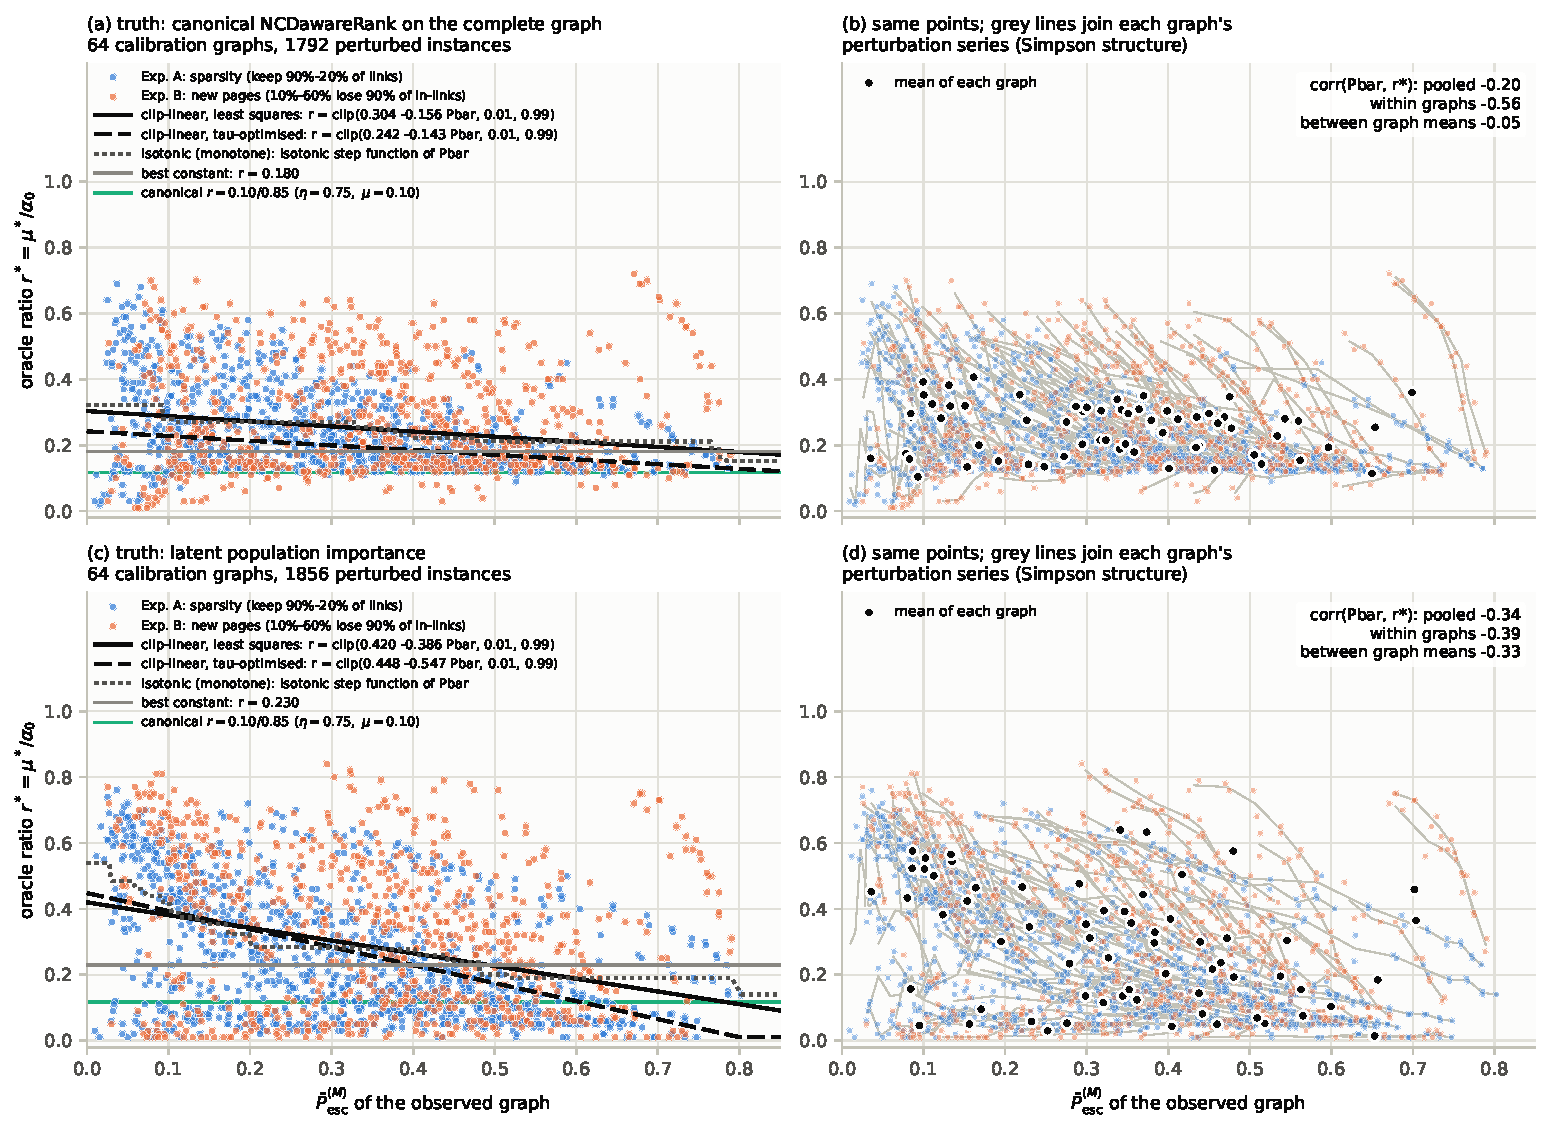
\includegraphics[width=\textwidth]{stage1_calibration_scatter.pdf}
\caption{Stage~1: oracle ratio $r^*$ against $\Pbar$ of the observed graph on the calibration panel.
\textbf{(a)} Truth NCD with the fitted candidate rules and the canonical $r$. \textbf{(c)} Truth POP.
\textbf{(b,\,d)} The same points, with grey lines joining the perturbation series of each graph and black
dots marking graph means. The pooled slope is a mixture of a steep within-graph relation and an almost
flat between-graph one.}
\label{fig:s1scatter}
\end{figure}

\subsection{Why \texorpdfstring{$\Pbar$}{P̄} does not transfer: Simpson structure}
The pooled correlation between $\Pbar$ and $r^*$ is \SOnePooled. Within graphs it is \SOneWithin{}
(\SOneWithinA{} in Experiment~A and \SOneWithinB{} in Experiment~B), and between graph means it is
\SOneBetween. Inside a graph, $\Pbar$ simply tracks how many links the perturbation removed: its
within-graph correlation with the fraction of arcs kept is \SOnePkeepA{} (A) and \SOnePkeepB{} (B).
Removing links lowers both $\Pbar$ and the agreement between observed and complete graph, and the
latter calls for more weight on the block-level smoothing of $M$. Across graphs, however, the level of
$\Pbar$ says almost nothing about $r^*$. A practitioner observes a single graph and cannot tell whether
a low $\Pbar$ comes from heavy link loss or from a naturally block-confined graph. The fitted slope is
therefore of little use out of sample.

\subsection{What determines \texorpdfstring{$r^*$}{r*}}
Table~\ref{tab:stage1dec} decomposes the variance of $r^*$ under each truth. Under NCD, graph identity
explains \SOneDecBase{} and the perturbation level \SOneDecLevel{}; additively they explain \SOneDecBL.
Boosted trees on the \emph{hidden} generator parameters plus the level recover \SOneDecHidden{} out of
sample, whereas every observable statistic together recovers $\SOneDecObs$ and $\Pbar$ alone
$\SOneDecP$. The graph-level component is associated with the latent quality structure. The graph mean
of $r^*$ correlates \SOneCorrICC{} with the ICC and \SOneCorrFit{} with the dispersion of latent quality
under NCD, and \SOneCorrICCPop{} and \SOneCorrFitPop{} under POP (Figure~\ref{fig:s1diag}c). This is
the regime in which shrinkage towards block averages, which is what
$M$ performs, pays off. Neither quantity is visible in global statistics of the observed graph. The
test--retest correlation of $r^*$ between replicates is \SOneRetest, so the unexplained part is not
noise in the oracle.

\begin{table}[t]
\centering
\footnotesize
\caption{Share of the variance of the oracle ratio $r^*$ explained ($R^2$) on the calibration panel. Graph identity, perturbation level and their additive combination are in-sample ANOVA shares. Starred columns are out of sample (grouped 8-fold CV by graph): boosted trees on the hidden generator parameters plus the perturbation level; ridge regression on every observable global statistic; and the clip-linear rule on $\bar P^{(M)}_{\mathrm{esc}}$. Negative values mean worse than predicting the mean.}
\label{tab:stage1dec}
\begin{tabular}{@{}lrrrrrr@{}}
\toprule
truth & graph & level & graph+level & hidden+level$^{*}$ & all observables$^{*}$ & $\bar P^{(M)}_{\mathrm{esc}}$ alone$^{*}$ \\
\midrule
NCD & 0.31 & 0.42 & 0.74 & 0.71 & -0.01 & 0.03 \\
PR & 0.41 & 0.30 & 0.71 & 0.70 & -0.08 & -0.02 \\
POP & 0.74 & 0.13 & 0.87 & 0.63 & 0.11 & 0.07 \\
SELF & 0.34 & 0.04 & 0.38 & -0.36 & -0.02 & 0.00 \\
\bottomrule
\end{tabular}
\end{table}


\subsection{Sensitivity to the ground truth}
\label{sec:res1-truth}
Figure~\ref{fig:s1truth} repeats the analysis under all four truths. Under PR, \SOnePrLower\% of the
oracle ratios sit at the lower bound $r=0.01$, because a PageRank reference favours $r\to0$. Under POP,
the relation with $\Pbar$ is negative both within graphs (\SOnePopWithinT) and between graphs
(\SOnePopBetweenT), but the fitted rule still does not beat a constant out of sample
(Appendix Table~\ref{tab:stage1truth}). Under SELF, the protocol of~\cite{ng13}, \SOneSelfUpper\%
of the oracle ratios sit at the upper bound $r=0.99$. Comparing a ranking with \emph{its own}
complete-graph ranking rewards whatever makes the ranking insensitive to links: large $r$ smooths rank
over blocks, which are not perturbed. The same holds for $\alpha$: as $\alpha\to0$, both rankings tend
to $v$, which depends only on the partition, so $\tau\to1$. Stability is a legitimate property to
report, but it cannot serve as a target for choosing parameters.

\begin{figure}[t]
\centering
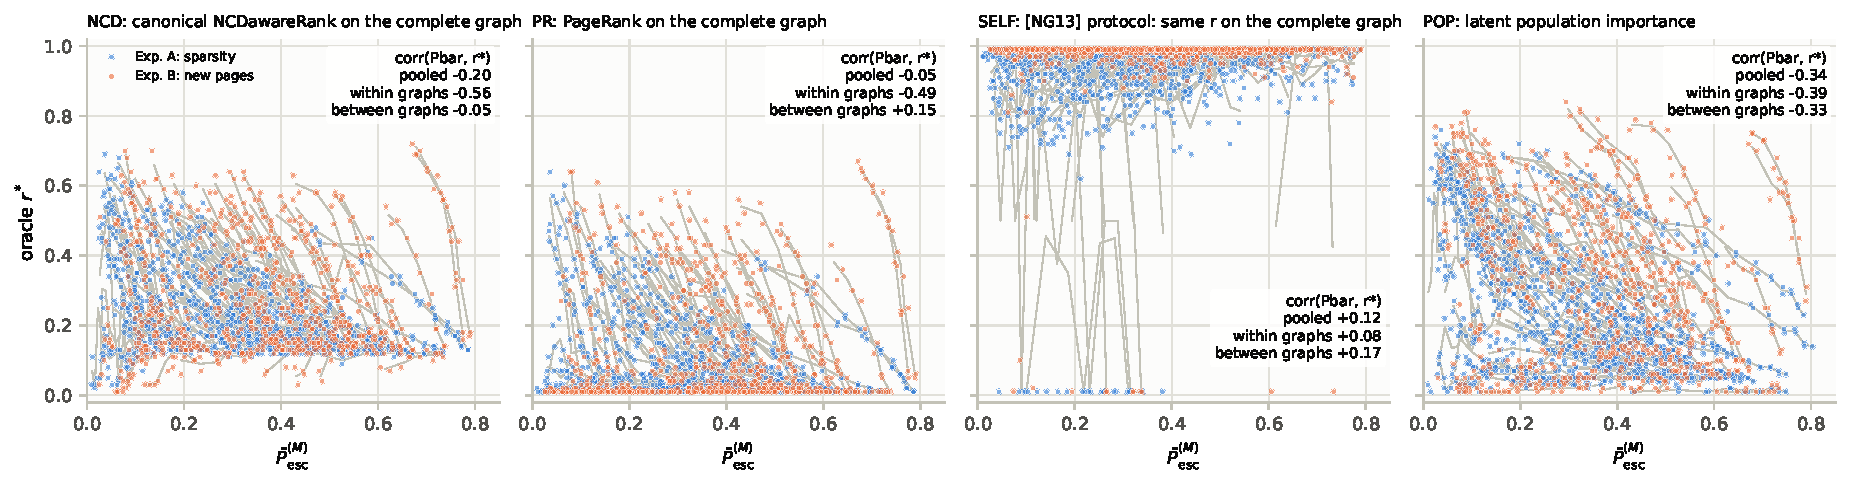
\includegraphics[width=\textwidth]{stage1_gt_sensitivity.pdf}
\caption{Stage~1 oracle ratio against $\Pbar$ under the four truths of Stage~1 (calibration panel).
Under SELF, the protocol of~\cite{ng13}, the oracle is pushed to the upper bound of the grid.}
\label{fig:s1truth}
\end{figure}

\begin{figure}[t]
\centering
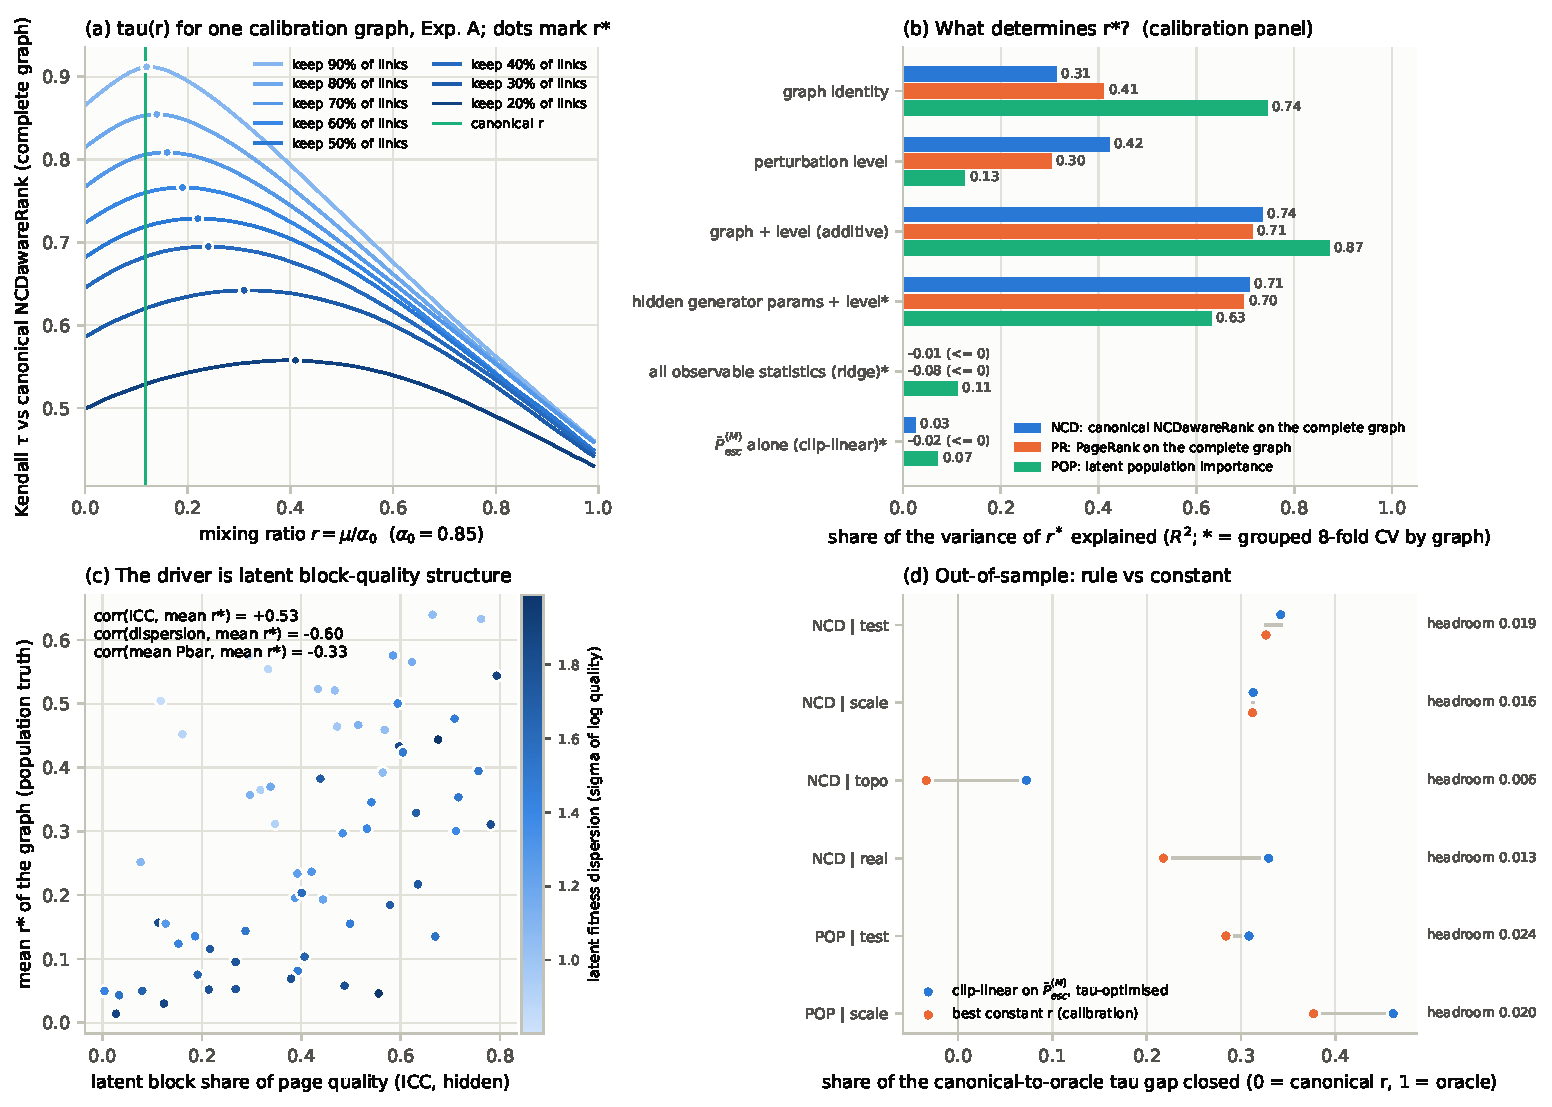
\includegraphics[width=\textwidth]{stage1_diagnostics.pdf}
\caption{Stage~1 diagnostics. \textbf{(a)} $\tau(r)$ curves for one calibration graph under increasing
link loss; dots mark $r^*$, which moves away from the canonical value as links disappear.
\textbf{(b)} Share of the variance of $r^*$ explained by each source. \textbf{(c)} Graph-mean $r^*$
under POP against the latent ICC, coloured by the dispersion of latent quality. \textbf{(d)} Share of
the canonical-to-oracle gap closed out of sample by the rule and by the best constant.}
\label{fig:s1diag}
\end{figure}

\subsection{Real networks}
Per graph, the Stage~1 rule changes $\tau$ relative to the canonical setting by \SOneRealCiteseer{}
(CiteSeer), \SOneRealCnr{} (cnr-2000), \SOneRealCorafull{} (Cora), \SOneRealCoraml{} (Cora-ML) and
\SOneRealWikics{} (WikiCS). The panel-level gain comes from CiteSeer alone, a very sparse graph (mean
out-degree $1.27$) whose arcs fall $95\%$ inside blocks. The fitted rule is also extrapolated there:
CiteSeer's $\Pbar=\PbarCiteseer$ lies at the edge of the calibration range. On cnr-2000
($\Pbar=\PbarCnr$) the rule prescribes $r=\RuleRCnr$, i.e.\ $\mu=\RuleMuCnr$ at $\alpha=0.85$, about
twice the canonical $\mu$, and loses $\tau$ against it. The rule returns $r\approx0.12$ only for
$\Pbar\approx0.85$, a value no real graph in this study approaches.

\FloatBarrier
% =============================================================================
\section{Results: Stage~2, the total damping}
\label{sec:res2}

\subsection{Candidate rules}
Figure~\ref{fig:s2scatter}(a) plots the oracle damping $\alpha^*$ against $h$ for the calibration graphs,
with $r$ locked to the Stage~1 rule; Table~\ref{tab:stage2} reports every candidate. The oracle is
$\alpha^*=\STwoAstarMean\pm\STwoAstarSd$. The $\tau$-optimised clipped-linear rule converges to the
constant $\alpha=\clip(0.810-0.000\,h)=\STwoConstAlpha$: once rank agreement is the objective, the
slope on $h$ is driven to zero. Every candidate that does depend on $h$ is worse than the constant.
\begin{itemize}[leftmargin=1.4em,itemsep=0pt]
\item The least-squares rule $\clip(\STwoLSa\STwoLSb\,h)$ loses \STwoTestLSvsConst{} on \texttt{test}
($p=\STwoTestLSvsConstP$) and \STwoTopoLSvsConst{} on \texttt{topo} ($p=\STwoTopoLSvsConstP$).
\item The isotonic rule loses \STwoTestIsoVsConst{} ($p=\STwoTestIsoVsConstP$) on \texttt{test}.
\item The displacement-budget rule $c/(c+h)$, $c=\STwoBudgetC$, loses \STwoTestBudVsConst{} on
\texttt{test} and \STwoScaleBudVsConst{} on \texttt{scale}.
\item Boosted trees on every observable statistic, including $h$ and $h_v$, are the most flexible
candidate, yet they lose \STwoTopoGbmVsConst{} on \texttt{topo} ($p=\STwoTopoGbmVsConstP$).
\item Replacing $h$ by $h_v$ changes nothing (the least-squares rule $\clip(\STwoLSva\STwoLSvb\,h_v)$
loses \STwoTestLSvVsConst{} on \texttt{test}, $p=\STwoTestLSvVsConstP$).
\end{itemize}
The constant itself improves on $\alpha=0.85$ by \STwoTestConstVs{} on \texttt{test} ($p=\STwoTestConstP$),
\STwoScaleConstVs{} on \texttt{scale} and \STwoTopoConstVs{} on \texttt{topo}, closing \STwoTestConstGap\%,
\STwoScaleConstGap\% and \STwoTopoConstGap\% of the gap to the oracle. On \texttt{real} it changes $\tau$
by \STwoRealConstVs{} ($p=\STwoRealConstP$).

\begin{table*}[t]
\centering
\footnotesize
\caption{Stage~2 candidate rules $\alpha=g(h)$ and $\alpha=g(h_v)$ with $r$ locked to the Stage~1 rule, truth NCD. Top block: mean Kendall $\tau$ of the static damping, the locked constant, their difference and the oracle. Lower blocks: difference in mean $\tau$ of each fitted rule against the locked constant. CV $\tau$: grouped 8-fold cross-validation on the calibration graphs. $^{\dagger}$: Wilcoxon signed-rank $p<0.01$ over graphs. Every rule is clipped to $[0.40,0.99]$; LS: least squares on the oracle values; $\tau$-opt.: fitted by maximising the mean calibration $\tau$.}
\label{tab:stage2}
\begin{tabular}{@{}llrrrrr@{}}
\toprule
rule & formula & CV $\tau$ & \texttt{test} & \texttt{scale} & \texttt{topo} & \texttt{real} \\
\midrule
\multicolumn{7}{@{}l}{\emph{mean Kendall $\tau$}} \\
static $\alpha=0.85$ & & -- & 0.6867 & 0.6681 & 0.7844 & 0.7600 \\
constant $\alpha=0.810$ (locked) & & 0.6913 & 0.6911 & 0.6735 & 0.7875 & 0.7559 \\
\quad difference & &  & $+$0.0044$^{\dagger}$ & $+$0.0054$^{\dagger}$ & $+$0.0031$^{\dagger}$ & $-$0.0012 \\
oracle $\alpha^*$ & & -- & 0.6960 & 0.6787 & 0.7911 & 0.7738 \\
\midrule
\multicolumn{7}{@{}l}{\emph{rules on $h$: difference in mean $\tau$ against the locked constant}} \\
clip-linear, $\tau$-opt.\ (locked) & $\mathrm{clip}(0.810-0.000\,h)$ & 0.6912 & 0.0000 & 0.0000 & 0.0000 & 0.0000 \\
clip-linear, LS & $\mathrm{clip}(0.803-0.021\,h)$ & 0.6898 & $-$0.0015$^{\dagger}$ & $-$0.0013 & $-$0.0007$^{\dagger}$ & $-$0.0033 \\
isotonic & -- & 0.6897 & $-$0.0016$^{\dagger}$ & $-$0.0014 & $-$0.0010$^{\dagger}$ & $-$0.0049 \\
budget $c/(c+x)$, $\tau$-opt. & $c=2.69$ & 0.6891 & $-$0.0023$^{\dagger}$ & $-$0.0043$^{\dagger}$ & $-$0.0016$^{\dagger}$ & $-$0.0045 \\
boosted trees, all observables & -- & 0.6905 & $-$0.0002 & $-$0.0030 & $-$0.0018$^{\dagger}$ & $-$0.0124 \\
\midrule
\multicolumn{7}{@{}l}{\emph{rules on $h_v$: difference in mean $\tau$ against the locked constant}} \\
clip-linear, $\tau$-opt.\ (locked) & $\mathrm{clip}(0.810+0.000\,h_v)$ & 0.6912 & 0.0000 & 0.0000 & 0.0000 & 0.0000 \\
clip-linear, LS & $\mathrm{clip}(0.802-0.016\,h_v)$ & 0.6898 & $-$0.0015$^{\dagger}$ & $-$0.0013 & $-$0.0011$^{\dagger}$ & $-$0.0029 \\
isotonic & -- & 0.6896 & $-$0.0018$^{\dagger}$ & $-$0.0013 & $-$0.0024$^{\dagger}$ & $-$0.0037 \\
budget $c/(c+x)$, $\tau$-opt. & $c=3.04$ & 0.6888 & $-$0.0024 & $-$0.0037 & $-$0.0083$^{\dagger}$ & $-$0.0019 \\
\bottomrule
\end{tabular}
\end{table*}


\begin{figure}[p]
\centering
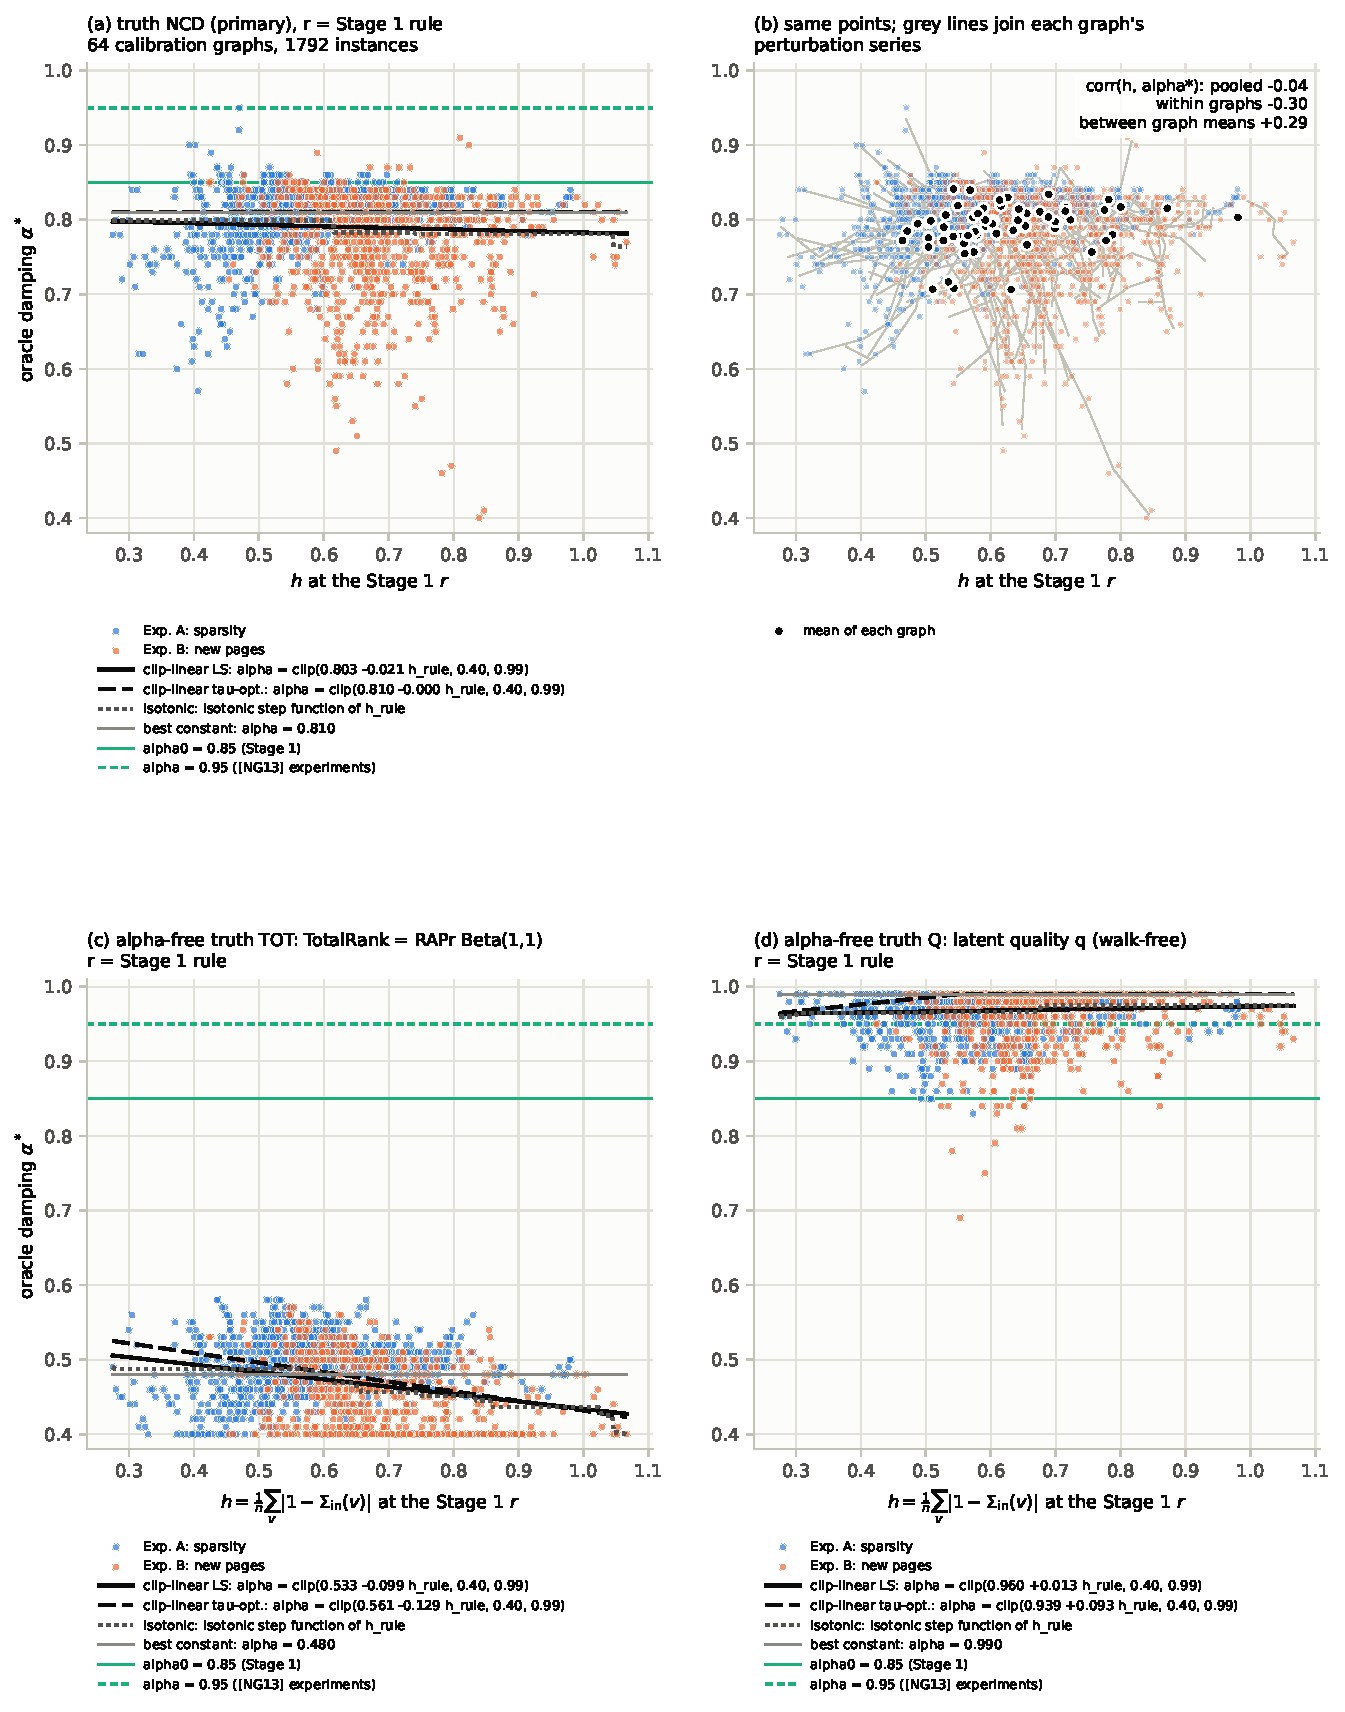
\includegraphics[width=0.94\textwidth]{stage2_calibration_scatter.pdf}
\caption{Stage~2: oracle damping $\alpha^*$ against $h$ (computed at the Stage~1 $r$) on the calibration
panel. \textbf{(a)} Primary truth NCD with the fitted candidates of $g$. The least-squares and
$\tau$-optimised fits are nearly flat, and the latter coincides with the constant $0.810$.
\textbf{(b)} The same points with each graph's perturbation series joined. \textbf{(c,\,d)} The two
$\alpha$-free truths, TOT ($\alpha^*\approx0.47$) and Q ($\alpha^*$ near the top of the grid).
Horizontal lines: $\alpha_0=0.85$ and the $\alpha=0.95$ of~\cite{ng13}.}
\label{fig:s2scatter}
\end{figure}

\subsection{Why \texorpdfstring{$h$}{h} cannot track \texorpdfstring{$\alpha^*$}{α*}}
\label{sec:hmech}
The pooled correlation between $h$ and $\alpha^*$ is \STwoPooled. Within graphs it is \STwoWithin, and
between graph means \STwoBetween{} (for $h_v$: \STwoWithinHv{} and \STwoBetweenHv). The within-graph
value is itself a mixture of two opposite mechanisms, one per perturbation:
\begin{itemize}[leftmargin=1.4em,itemsep=1pt]
\item \emph{Experiment~A (uniform link removal) lowers $h$.} The mean $h$ falls from \STwoHmildA{} at
$90\%$ of arcs kept to \STwoHsevereA{} at $20\%$ (within-graph correlation with the kept fraction
\STwoHkeepA). Removing arcs creates dangling pages, and their uniform rows add $n_{\mathrm d}/n$ to every
column sum, pulling $\Sin$ towards~$1$ (correlation of $h$ with the dangling fraction \STwoHdangA).
\item \emph{Experiment~B (newly added pages) raises $h$}, from \STwoHmildB{} to \STwoHsevereB{}: pages
that lose $90\%$ of their in-links acquire $\Sin\approx0$ (correlation of $h$ with the share of
zero-inflow pages \STwoHzinB).
\end{itemize}
In both experiments $\alpha^*$ \emph{decreases} with severity, from \STwoAmildA{} to \STwoAsevereA{} (A)
and from \STwoAmildB{} to \STwoAsevereB{} (B). The within-graph correlation of $h$ with $\alpha^*$ is
therefore \STwoHastarA{} under A and \STwoHastarB{} under B. A statistic that rises under one kind of
link loss and falls under the other, while the optimal damping falls under both, cannot calibrate
$\alpha$. The initial hypothesis that a larger $h$ calls for a larger $\alpha$ is contradicted, and so
is its opposite. Table~\ref{tab:stage2dec} quantifies this. Under NCD, $h$ alone explains $\STwoDecH$ of
the variance of $\alpha^*$ out of sample, and at most \STwoDecHmax{} under any truth. Graph identity
explains \STwoDecBase{} and the perturbation level, which is not observable in practice, \STwoDecLevel;
boosted trees on the hidden generator parameters plus the level recover \STwoDecHidden{} out of sample,
whereas every observable statistic together recovers only \STwoDecObs.

\begin{table}[t]
\centering
\footnotesize
\caption{Share of the variance of the oracle damping $\alpha^*$ explained ($R^2$) on the calibration panel, for each truth and $r$-setting. Graph identity, perturbation level and their additive combination are in-sample ANOVA shares. Starred columns are out of sample (grouped 8-fold CV by graph): boosted trees on the hidden generator parameters plus the perturbation level; ridge regression on every observable global statistic, including $h$ and $h_v$; and the clip-linear rule on $h$ alone. Negative values mean worse than predicting the mean.}
\label{tab:stage2dec}
\begin{tabular}{@{}llrrrrrr@{}}
\toprule
truth & $r$ & graph & level & graph+level & hidden+level$^{*}$ & all observables$^{*}$ & $h$ alone$^{*}$ \\
\midrule
NCD & Stage~1 & 0.25 & 0.47 & 0.72 & 0.60 & 0.17 & $-$0.02 \\
NCD & 0.118 & 0.32 & 0.41 & 0.73 & 0.62 & 0.13 & $-$0.03 \\
NCD95 & 0.105 & 0.40 & 0.22 & 0.62 & 0.38 & 0.10 & $-$0.03 \\
TOT & Stage~1 & 0.10 & 0.77 & 0.87 & 0.87 & 0.18 & 0.05 \\
POP & POP rule & 0.54 & 0.29 & 0.83 & 0.44 & 0.28 & $-$0.03 \\
Q & Stage~1 & 0.67 & 0.02 & 0.69 & $-$0.20 & 0.05 & $-$0.03 \\
\bottomrule
\end{tabular}
\end{table}


\begin{table}[t]
\centering
\small
\caption{Experiments A and B are mixtures of dangling-page and zero-in-link effects. Values run from the least damaged to the most severe level.}
\label{tab:mixture}
\begin{tabular}{@{}lrrrr@{}}\toprule
experiment & $\delta$ & $\zeta$ & $h$ & $h_{\rm raw}$ \\
\midrule
A: link keep 1.0$\to$0.2 & 0.173$\to$0.483 & 0.156$\to$0.506 & 0.620$\to$0.476 & 0.679$\to$0.669 \\
B: page loss 0.1$\to$0.6 & 0.185$\to$0.298 & 0.207$\to$0.461 & 0.644$\to$0.704 & 0.707$\to$0.827 \\
\bottomrule\end{tabular}
\end{table}


Experiments A and B are mixtures of dangling-page creation, zero-in-link pages and altered
transition mass, with different proportions. The generated table makes this composition explicit.
In particular, $h_{\rm raw}$ alone is nearly blind to A, so it is not a general-purpose severity
measure for both perturbation protocols.

\paragraph{Non-monotone and dangling-deconfounded rules.}
Because $\alpha^*$ falls under both perturbations while $h$ moves in opposite directions, within one
graph $\alpha^*$ is an inverted V in $h$ around the graph's unperturbed value $h_0$ (the joined series in
Figure~\ref{fig:s2scatter}b). The distance from that apex carries real information: $|h-h_0|$
correlates \NmDistOwn{} with $\alpha^*$ (\NmDistOwnWithin{} within graphs). We therefore searched for a
rule that exploits the shape (script \texttt{stage2\_nonmonotone\_search.py}; Table~\ref{tab:nonmono}).
Asymmetric tents
$\clip\bigl(\alpha_{\mathrm{peak}}-s_L\max(0,h_0-h)-s_R\max(0,h-h_0),\,0.40,\,0.99\bigr)$, symmetric
tents, a concave quadratic, a Gaussian bump, two- and three-region step functions and a two-knot linear
spline were fitted on $h$ and on $h_v$, both by least squares to $\alpha^*$ and by direct maximisation
of mean $\tau$ (exactly for the step functions; otherwise by grid search, with the apex of rules on
$h$ in $[0.50,0.70]$, followed by Nelder--Mead and Powell). They were
evaluated exactly as the other candidates: 8-fold cross-validation by graph on \texttt{calib}, with the
constant refitted in every fold, then the four held-out panels. The $\tau$-optimised tent places its
apex at $h_0=\NmTentHzero$, with $\alpha_{\mathrm{peak}}=\NmTentPeak$, $s_L=\NmTentSL$ and
$s_R=\NmTentSR$. It does follow part of the within-graph variation (its predictions correlate
\NmTentWithin{} with $\alpha^*$ within graphs), yet it changes mean $\tau$ by only \NmTentCalib{} in
sample, \NmTentCV{} in cross-validation ($p=\NmTentCVP$) and \NmTentHeld{} on the 73 held-out graphs
($p=\NmTentHeldP$). No $\tau$-optimised non-monotone rule on $h$ or $h_v$ gains more than
\NmMaxOneDCV{} in cross-validation or \NmMaxOneDHeld{} out of sample, and the least-squares fits change
$\tau$ by \NmLSBest{} to \NmLSWorst{} out of sample.

Removing the uniform dangling contribution $(1-r)\,\delta$, with $\delta=n_{\mathrm d}/n$, from every
column sum tests whether the fall of $h$ under Experiment~A is a dangling artefact. Largely it is: the
deconfounded deviation $h_{\mathrm{raw}}=\frac1n\sum_v|1-\Sin(v)+(1-r)\delta|$ barely moves under A
(\NmHrawFull{} unperturbed, \NmHrawSevA{} at $20\%$ of arcs kept) and rises under B (\NmHrawSevB{} at
$60\%$). Two further variants rise under both perturbations: the relative dispersion
$h_{\mathrm{raw}}^{\mathrm{rel}}$ of the deconfounded sums (from \NmHrelFull{} to \NmHrelSevA{} under A
and \NmHrelSevB{} under B) and the deviation $h_{\mathrm{raw}}^{H}$ of the column sums of the hyperlink
matrix before its dangling rows are patched (from \NmHHFull{} to \NmHHSevA{} and \NmHHSevB). Within
graphs, both correlate negatively with $\alpha^*$ under each experiment (\NmHrelAstarA{} and
\NmHrelAstarB{} for $h_{\mathrm{raw}}^{\mathrm{rel}}$). Deconfounding thus turns the inverted V into a
monotone relation, but only inside each graph. The unperturbed level of $h_{\mathrm{raw}}^{\mathrm{rel}}$
varies across graphs with standard deviation \NmRelSd, against within-graph excursions of \NmRelExcA{}
(A) and \NmRelExcB{} (B), and it correlates \emph{positively} with the graph-mean $\alpha^*$
(\NmRelBetween): the Simpson structure of Stage~1 again. The $\tau$-optimised tents on the three
deconfounded statistics degenerate to a decreasing hinge, and no rule on them gains more than
\NmRawMaxCV{} in cross-validation or \NmRawMaxHeld{} out of sample.

The two raw counts that rise under both perturbations give the strongest deployable rules: the dangling
fraction $\delta$ (from \NmDangFull{} to \NmDangSevA{} under A and \NmDangSevB{} under B; Experiment~B
also creates dangling pages, because it deletes the out-arcs of pages whose links all pointed to the new
pages) and the share $\zeta$ of pages without in-links (from \NmZinFull{} to \NmZinSevA{} and
\NmZinSevB). The bivariate rule $\clip(\NmBilinDeltaA\NmBilinDeltaH\,h\NmBilinDeltaD\,\delta)$ gains
\NmBilinCV{} in cross-validation ($p=\NmBilinCVP$) but \NmBilinHeld{} out of sample
($p=\NmBilinHeldP$). The clipped-linear rule $\alpha=\clip(\NmZetaA\NmZetaB\,\zeta)$ gains \NmZetaCV{}
in cross-validation ($p=\NmZetaCVP$) and \NmZetaHeld{} on the held-out graphs ($p=\NmZetaHeldP$);
adding $h$ leaves it unchanged (coefficient \NmBilinZetaH). Its gain comes from the two panels drawn from
the calibration generator (\NmZetaTest{} on \texttt{test}, \NmZetaScale{} on \texttt{scale}), shrinks to
\NmZetaTopo{} on \texttt{topo} and reverses on \texttt{real} (\NmZetaReal, worse on three of the five
graphs). The unperturbed share of pages without in-links is \NmZinUnpertCalib{} on \texttt{calib} but
\NmZinUnpertTopo{} on \texttt{topo} and \NmZinUnpertReal{} on \texttt{real} (\NmZinCiteMin--\NmZinCiteMax{}
on the three citation graphs), so its level, too, mixes the graph with the perturbation.

The obstacle is the location of the apex, not the shape of $g$. Given each graph's own unperturbed $h_0$,
which the observed graph does not reveal, a $\tau$-optimised tent in $h-h_0$ gains \NmDhCV{} in
cross-validation ($p=\NmDhCVP$; \NmDhShare\% of the oracle headroom of \NmOracleCalib) and \NmDhHeld{}
out of sample ($p=\NmDhHeldP$). A step rule in $h_{\mathrm{raw}}-h_{\mathrm{raw},0}$ gains \NmDhrawHeld{}
out of sample ($p=\NmDhrawHeldP$), on all four held-out panels. With one apex for every graph, the
correlation of $\alpha^*$ with the distance falls from \NmDistOwn{} to \NmDistGlobal{} (best common apex
\NmDistGlobalC): the apex varies across graphs with standard deviation \NmHzeroSd, as much as $h$ moves
within a graph under the perturbations (mean excursions \NmExcA{} under A and \NmExcB{} under B). None of the \NmRules{} deployable
rules meets the decision rule fixed before the held-out evaluation: a gain of at least $0.0005$ with
$p<0.05$ both in cross-validation and on the pooled held-out panels, and no Holm-significant loss on any
panel. The cross-validation part is passed by \NmMeetsCV{} rules, the held-out part by none. The constant
$\alpha=\STwoConstAlpha$ therefore remains the Stage~2 rule. The same search under NCD95 (constant
\NmNfConst) and TOT (constant \NmTotConst) promotes no rule either, while the tent in $h-h_0$ is again
significant out of sample (\NmNfDhHeld, $p=\NmNfDhHeldP$, and \NmTotDhHeld, $p=\NmTotDhHeldP$).

\begin{table}[t]
\centering
\footnotesize\setlength{\tabcolsep}{4pt}
\caption{Non-monotone, dangling-deconfounded and bivariate Stage~2 rules against the locked constant $\alpha=0.810$ (truth NCD, $r$ = Stage~1 rule), selected from the 127 deployable rules of \texttt{stage2\_nonmonotone\_search.py}. Entries are differences in mean Kendall $\tau$ in units of $10^{-4}$, rule minus constant (the decision threshold $0.0005$ is $5.0$). calib: in sample; CV: grouped 8-fold cross-validation on \texttt{calib}, with the constant refitted in every fold; held-out: the 73 graphs of \texttt{test}, \texttt{scale}, \texttt{topo} and \texttt{real} pooled. $p$: Wilcoxon signed-rank test over per-graph means; $^{\dagger}$: Holm-adjusted $p<0.05$ across the four panels. Rules are $\tau$-optimised unless marked LS. $h_0$ and $h_{\mathrm{raw},0}$ are the values on the graph's own unperturbed version; the two ceilings are in sample.}
\label{tab:nonmono}
\begin{tabular}{@{}lrrrrrrrrr@{}}
\toprule
rule & calib & CV & $p_{\mathrm{CV}}$ & held-out & $p$ & \texttt{test} & \texttt{scale} & \texttt{topo} & \texttt{real} \\
\midrule
\multicolumn{10}{@{}l}{\emph{non-monotone rules on $h$ and $h_v$}} \\
\quad asymmetric tent, LS & $-$11.8 & $-$14.5 & $3.9\times10^{-4}$ & $-$16.6 & $2.6\times10^{-7}$ & $-$17.7$^{\dagger}$ & $-$17.5 & $-$7.2$^{\dagger}$ & $-$52.4 \\
\quad asymmetric tent & $+$0.9 & $-$1.0 & 0.538 & $-$1.1 & 0.290 & $-$1.2 & $-$3.3 & $-$0.1 & $-$0.6 \\
\quad symmetric tent & $+$0.3 & $-$1.8 & 0.412 & $-$0.7 & 0.477 & $+$0.0 & $-$2.2 & $-$0.8 & $-$0.7 \\
\quad concave quadratic & 0.0 & $-$1.9 & 0.072 & 0.0 & -- & 0.0 & 0.0 & 0.0 & 0.0 \\
\quad Gaussian bump & $+$1.3 & $+$0.1 & 0.915 & $+$0.4 & 0.263 & $+$0.5 & $-$2.6 & $+$0.1 & $+$8.8 \\
\quad three-region step & $+$1.7 & $+$0.5 & 0.586 & $-$0.8 & 0.166 & $-$1.5 & $-$2.4 & $+$0.2 & $+$2.3 \\
\quad two-knot linear spline & $+$1.4 & $-$0.8 & 0.963 & $-$0.1 & 0.343 & $-$0.3 & $-$2.2 & $+$0.1 & $+$5.0 \\
\quad asymmetric tent on $h_v$ & $+$0.0 & $-$2.4 & 0.784 & $-$0.2 & 0.245 & $-$0.2 & $+$0.1 & $-$0.0 & $-$1.7 \\
\multicolumn{10}{@{}l}{\emph{dangling-deconfounded and severity statistics}} \\
\quad tent on $h_{\mathrm{raw}}$ & $+$1.0 & $-$0.3 & 0.108 & $+$1.0 & 0.245 & $+$3.0$^{\dagger}$ & $-$0.0 & $-$1.3 & $+$1.7 \\
\quad tent on $h_{\mathrm{raw}}^{\mathrm{rel}}$ & $+$3.2 & $+$1.6 & 0.009 & $+$1.2 & 0.366 & $+$5.1$^{\dagger}$ & $+$1.6 & $-$3.1 & $-$4.9 \\
\quad tent on $h_{\mathrm{raw}}^{H}$ & $+$3.5 & $+$2.1 & 0.008 & $+$0.9 & 0.562 & $+$5.2$^{\dagger}$ & $+$1.7 & $-$0.0$^{\dagger}$ & $-$24.7 \\
\quad two-region step on $\delta$ & $+$4.8 & $+$4.5 & $2.0\times10^{-5}$ & $+$3.0 & 0.005 & $+$3.8$^{\dagger}$ & $+$7.5 & $-$1.3 & $+$8.2 \\
\quad clipped-linear on $\zeta$ & $+$15.0 & $+$14.2 & $2.0\times10^{-7}$ & $+$3.1 & 0.039 & $+$9.0$^{\dagger}$ & $+$12.4 & $+$3.8 & $-$59.6 \\
\quad three-region step on $\zeta$ & $+$13.7 & $+$10.3 & $3.9\times10^{-5}$ & $+$4.0 & 0.014 & $+$8.2$^{\dagger}$ & $+$12.0 & $+$0.7 & $-$26.4 \\
\multicolumn{10}{@{}l}{\emph{bivariate rules}} \\
\quad clipped-linear in $(h,\delta)$ & $+$8.4 & $+$6.6 & 0.001 & $+$3.5 & 0.119 & $+$6.4 & $+$12.0 & $-$3.3 & $-$2.4 \\
\quad tent in $h$ $+\,c\,\delta$ & $+$8.3 & $+$6.4 & 0.002 & $+$3.2 & 0.155 & $+$5.8 & $+$11.0 & $-$3.4 & $-$0.1 \\
\quad $3\times3$ cells in $(h,\delta)$ & $+$9.0 & $+$6.6 & $2.5\times10^{-4}$ & $+$1.5 & 0.297 & $+$6.3$^{\dagger}$ & $+$3.9 & $-$4.8 & $-$5.7 \\
\quad boosted trees on $(h,\delta)$, LS & $+$16.7 & $-$21.2 & 0.101 & $-$22.8 & $3.3\times10^{-4}$ & $-$10.8 & $-$16.4 & $-$20.9$^{\dagger}$ & $-$125.0 \\
\quad clipped-linear in $(h,\zeta)$ & $+$15.0 & $+$13.7 & $7.2\times10^{-7}$ & $+$3.3 & 0.046 & $+$9.0 & $+$12.3 & $+$4.4 & $-$60.1 \\
\multicolumn{10}{@{}l}{\emph{not deployable: need the unperturbed graph or the truth}} \\
\quad tent in $h-h_0$ & $+$19.2 & $+$17.8 & $7.0\times10^{-7}$ & $+$5.7 & 0.018 & $+$9.7 & $+$11.0 & $+$2.7 & $-$18.4 \\
\quad three-region step in $h_{\mathrm{raw}}-h_{\mathrm{raw},0}$ & $+$17.3 & $+$15.5 & $4.3\times10^{-7}$ & $+$9.7 & $6.1\times10^{-5}$ & $+$11.6$^{\dagger}$ & $+$13.3 & $+$3.5 & $+$18.9 \\
\quad best constant per graph & $+$9.1 & -- & -- & $+$15.4 & -- & $+$8.2 & $+$10.8 & $+$11.3 & $+$92.3 \\
\quad oracle $\alpha^*$ & $+$52.2 & -- & -- & $+$53.3 & -- & $+$48.6 & $+$52.1 & $+$35.6 & $+$171.9 \\
\bottomrule
\end{tabular}
\end{table}


\subsection{Anchoring and the noise discount}
\label{sec:anchor}
Table~\ref{tab:anchor} and Figure~\ref{fig:s2diag}(a,\,b) show the effect that dominates Stage~2: the
oracle damping is set by the reference ranking. On the unperturbed graph, the oracle equals the damping
that defines the truth: \AnchorNcd{} for NCD ($0.85$) and \AnchorNcdnf{} for NCD95 ($0.95$). It is
\AnchorTot{} for TOT, whose Beta(1,1) prior has mean $0.5$, \AnchorPop{} for POP and \AnchorQ{} for the
walk-free Q. Under perturbation it sits slightly lower: \MeanNcd, \MeanNcdnf, \MeanTot, \MeanPop{} and
\MeanQ{} respectively. POP is the only truth whose anchor lies clearly below its own damping even on the
unperturbed graph. This is expected: POP is defined on the generator's expected walk, and every realised
graph is already a noisy copy of that walk before any link is removed. The two $\alpha$-free references
disagree completely, TOT pointing to
$\alpha\approx0.5$ and Q to the top of the grid. For Q the optimum lies at the top of the grid rather
than beyond it: on \QupGraphs{} graphs, mean $\tau$ against $q$ is \QupNine, \QupNineFive{} and
\QupNineNine{} at $\alpha=0.99$, $0.995$ and $0.999$.

\begin{table}[t]
\centering
\footnotesize
\caption{Oracle damping under the five truths (calibration panel). Own $\alpha$: the damping that defines the truth ($^{a}$TotalRank: mean of the Beta(1,1) prior; $^{b}$POP is the PageRank of the expected walk at $0.85$). $\alpha^*$ (A1.0): mean oracle on the unperturbed graphs. Mean $\alpha^*$: mean over the perturbed instances; discount: their difference. Const $\alpha$: the best constant on the calibration panel. Within/between: correlation of $h$ with $\alpha^*$ inside graphs and between graph means.}
\label{tab:anchor}
\begin{tabular}{@{}llrrrrrrr@{}}
\toprule
truth & $r$ & own $\alpha$ & $\alpha^*$ (A1.0) & mean $\alpha^*$ & discount & const $\alpha$ & within & between \\
\midrule
NCD & Stage~1 & 0.85 & 0.852 & 0.791 & $-$0.061 & 0.81 & $-$0.30 & $+$0.29 \\
NCD95 & 0.105 & 0.95 & 0.950 & 0.914 & $-$0.036 & 0.93 & $-$0.22 & $+$0.26 \\
TOT & Stage~1 & 0.50$^{a}$ & 0.547 & 0.471 & $-$0.075 & 0.48 & $-$0.37 & $-$0.15 \\
POP & POP rule & 0.85$^{b}$ & 0.767 & 0.726 & $-$0.042 & 0.74 & $-$0.54 & $+$0.14 \\
Q & Stage~1 & -- & 0.971 & 0.968 & $-$0.003 & 0.99 & $-$0.19 & $+$0.18 \\
\bottomrule
\end{tabular}
\end{table}


The dose-response test in Table~\ref{tab:rapr} isolates the mechanism. We vary the prior of
Random-$\alpha$ NCDawareRank references and nothing else. The mean oracle damping then follows the prior
mean with slope \RaprSlope{} (intercept \RaprIcpt): \RaprLo, \RaprMid, \RaprHi{} and \RaprTop{} for
prior means $0.30$, $0.50$, $0.70$ and $0.85$. The offset of $-0.03$ to $-0.06$ is the \emph{noise
discount}: when the observed graph is a perturbed copy of the reference graph, the best single damping
is slightly lower than the reference's own. The natural interpretation is that long walks propagate the
noise introduced by missing links, so a slightly shorter effective walk recovers the reference better.
Stage~2's move from $0.85$
to \STwoConstAlpha{} under NCD is exactly this effect. Under NCD95 the corresponding constant is
\NfConstAlpha, which improves on $\alpha=0.95$ by \NfTestD{} on \texttt{test} ($p=\NfTestP$),
\NfScaleD{} on \texttt{scale}, \NfTopoD{} on \texttt{topo} ($p=\NfTopoP$) and \NfRealD{} on
\texttt{real}.

\begin{table}[t]
\centering
\small
\caption{Dose-response test of anchoring: oracle damping $\alpha^*$ against Random-$\alpha$ NCDawareRank references $\mathbb{E}[\pi(A)]$ with $A\sim\mathrm{Beta}(a,b)$, on 16 calibration graphs (perturbed instances only, $r$ = Stage~1 rule, grid $0.05$--$0.99$). Beta(1,1) is TotalRank.}
\label{tab:rapr}
\begin{tabular}{@{}lrrrr@{}}
\toprule
prior & prior mean & mean $\alpha^*$ & s.d. & $\alpha^*-$mean \\
\midrule
Beta(3,7) & 0.30 & 0.267 & 0.046 & $-$0.033 \\
Beta(5,5) & 0.50 & 0.447 & 0.060 & $-$0.053 \\
Beta(1,1) & 0.50 & 0.460 & 0.062 & $-$0.040 \\
Beta(7,3) & 0.70 & 0.636 & 0.063 & $-$0.064 \\
Beta(8.5,1.5) & 0.85 & 0.793 & 0.056 & $-$0.057 \\
\bottomrule
\end{tabular}
\end{table}


The anchor-matched operational claim is conditional on the reference: use $\alpha=0.81$ when the
reference is defined at $0.85$, and $\alpha=0.93$ when it is defined at $0.95$. The first changes
the NCD comparison by \WpZeroNcdVsCanonical{}, while the matched NCD95 comparison changes by
\WpZeroNfMatched{} ($p=\WpZeroNfMatchedP$), a tie on \texttt{test}. The reference damping is a
methodological decision, and Table~\ref{tab:mismatch} shows what a mismatch costs on \texttt{test}: under
the NCD truth, a user whose reference is the canonical $(0.118,\,0.85)$ and who adopts the $0.95$-anchored
constant changes $\tau$ by \MisNcdNgHiCan{}; under the NCD95 truth, a user whose reference is
$(0.105,\,0.95)$ and who adopts $\alpha=0.81$ changes it by \MisNcdnfRuleLoNg{}.
With the Stage~1 rule in place of $r=0.105$, the same constant $0.93$ improves on the [NG13] setting
$(0.105,\,0.95)$ by \MisNcdnfRuleHiNg{} on \texttt{test} (\MisNcdnfRuleHiNgWins{} graphs, $p=\MisNcdnfRuleHiNgP$);
the best constant for that pairing on \texttt{calib} is \MisRuleBestCalib{}, and its $\tau$ exceeds
that of $0.93$ by only \MisRuleBestCalibGap{}. The two-stage pipeline also beats the [NG13] ranking setting $(0.105,\,0.95)$ by \WpZeroNcdVsNg{}
under the NCD truth, but that number mostly reflects the fact that the NCD truth is itself defined at
the damping $0.85$; it is not evidence about the method and is not used in any claim.

\begin{center}
\fbox{\begin{minipage}{0.94\linewidth}
\textbf{Practical recipe.} Choose the reference anchor first. For $0.85$, call
\texttt{tune(..., alpha\_ref=0.85)}: it returns Stage~1 $r$ and $\alpha=0.81$.
For $0.95$, use \texttt{alpha\_ref=0.95}: it returns the same Stage~1 $r$ and $\alpha=0.93$.
The calibration optimum for this pairing is \MisRuleBestCalib{}, only
\MisRuleBestCalibGap{} $\tau$ above $0.93$. The tool does not return the reference's own
$r=0.10/\alpha_{\rm ref}$; it returns Stage~1 $r$ by design. A baseline argument is ignored
with a warning because no baseline rule is validated.
\end{minipage}}
\end{center}

\begin{table*}[t]
\centering
\scriptsize
\caption{Anchor matching. Mean Kendall $\tau$ difference (candidate minus comparator), averaged over graphs, with graph wins in parentheses, on the four held-out panels; $^{\dagger}$ marks an exact Wilcoxon $p\ge0.05$ (every other cell has $p\le0.0269$). The comparators are the static [NG13] settings $(r,\alpha)$. Cells marked $^{\star}$ are the anchor-matched comparisons claimed in the text; the others are deliberate mismatches, in which the candidate, the comparator or the truth is defined at the other damping. With five real graphs the smallest attainable $p$ is $0.0625$.}
\label{tab:mismatch}
\begin{tabular}{@{}lcccc@{}}
\toprule
candidate $(r,\alpha)$ vs comparator & \texttt{test} & \texttt{scale} & \texttt{topo} & \texttt{real} \\
\midrule
\multicolumn{5}{@{}l}{\textit{truth NCD}} \\
\quad rule $r$, $\alpha=0.81$ vs $(0.118,\,0.85)$$^{\star}$ & $+$0.0110 (31/32) & $+$0.0102 (11/12) & $+$0.0036 (23/24) & $+$0.0017 (2/5)$^{\dagger}$ \\
\quad rule $r$, $\alpha=0.81$ vs $(0.105,\,0.95)$ & $+$0.0743 (32/32) & $+$0.0756 (12/12) & $+$0.0515 (24/24) & $+$0.0848 (5/5)$^{\dagger}$ \\
\quad rule $r$, $\alpha=0.93$ vs $(0.118,\,0.85)$ & $-$0.0414 (0/32) & $-$0.0472 (0/12) & $-$0.0318 (0/24) & $-$0.0777 (0/5)$^{\dagger}$ \\
\quad rule $r$, $\alpha=0.93$ vs $(0.105,\,0.95)$ & $+$0.0219 (31/32) & $+$0.0182 (11/12) & $+$0.0162 (24/24) & $+$0.0053 (4/5)$^{\dagger}$ \\
\quad $r=0.105$, $\alpha=0.93$ vs $(0.118,\,0.85)$ & $-$0.0441 (0/32) & $-$0.0455 (0/12) & $-$0.0300 (0/24) & $-$0.0528 (0/5)$^{\dagger}$ \\
\quad $r=0.105$, $\alpha=0.93$ vs $(0.105,\,0.95)$ & $+$0.0192 (32/32) & $+$0.0199 (12/12) & $+$0.0180 (24/24) & $+$0.0303 (5/5)$^{\dagger}$ \\
\multicolumn{5}{@{}l}{\textit{truth NCD95}} \\
\quad rule $r$, $\alpha=0.81$ vs $(0.118,\,0.85)$ & $-$0.0109 (6/32) & $-$0.0124 (2/12) & $-$0.0069 (2/24) & $-$0.0206 (0/5)$^{\dagger}$ \\
\quad rule $r$, $\alpha=0.81$ vs $(0.105,\,0.95)$ & $-$0.0303 (2/32) & $-$0.0306 (1/12) & $-$0.0172 (1/24) & $-$0.0654 (0/5)$^{\dagger}$ \\
\quad rule $r$, $\alpha=0.93$ vs $(0.118,\,0.85)$ & $+$0.0283 (31/32) & $+$0.0245 (10/12) & $+$0.0137 (21/24) & $+$0.0424 (5/5)$^{\dagger}$ \\
\quad rule $r$, $\alpha=0.93$ vs $(0.105,\,0.95)$$^{\star}$ & $+$0.0089 (30/32) & $+$0.0062 (10/12) & $+$0.0034 (20/24) & $-$0.0025 (1/5)$^{\dagger}$ \\
\quad $r=0.105$, $\alpha=0.93$ vs $(0.118,\,0.85)$ & $+$0.0205 (32/32) & $+$0.0197 (11/12) & $+$0.0130 (23/24) & $+$0.0443 (5/5)$^{\dagger}$ \\
\quad $r=0.105$, $\alpha=0.93$ vs $(0.105,\,0.95)$$^{\star}$ & $+$0.0011 (19/32)$^{\dagger}$ & $+$0.0015 (7/12)$^{\dagger}$ & $+$0.0026 (20/24) & $-$0.0006 (2/5)$^{\dagger}$ \\
\bottomrule
\end{tabular}
\end{table*}


\begin{figure}[t]
\centering
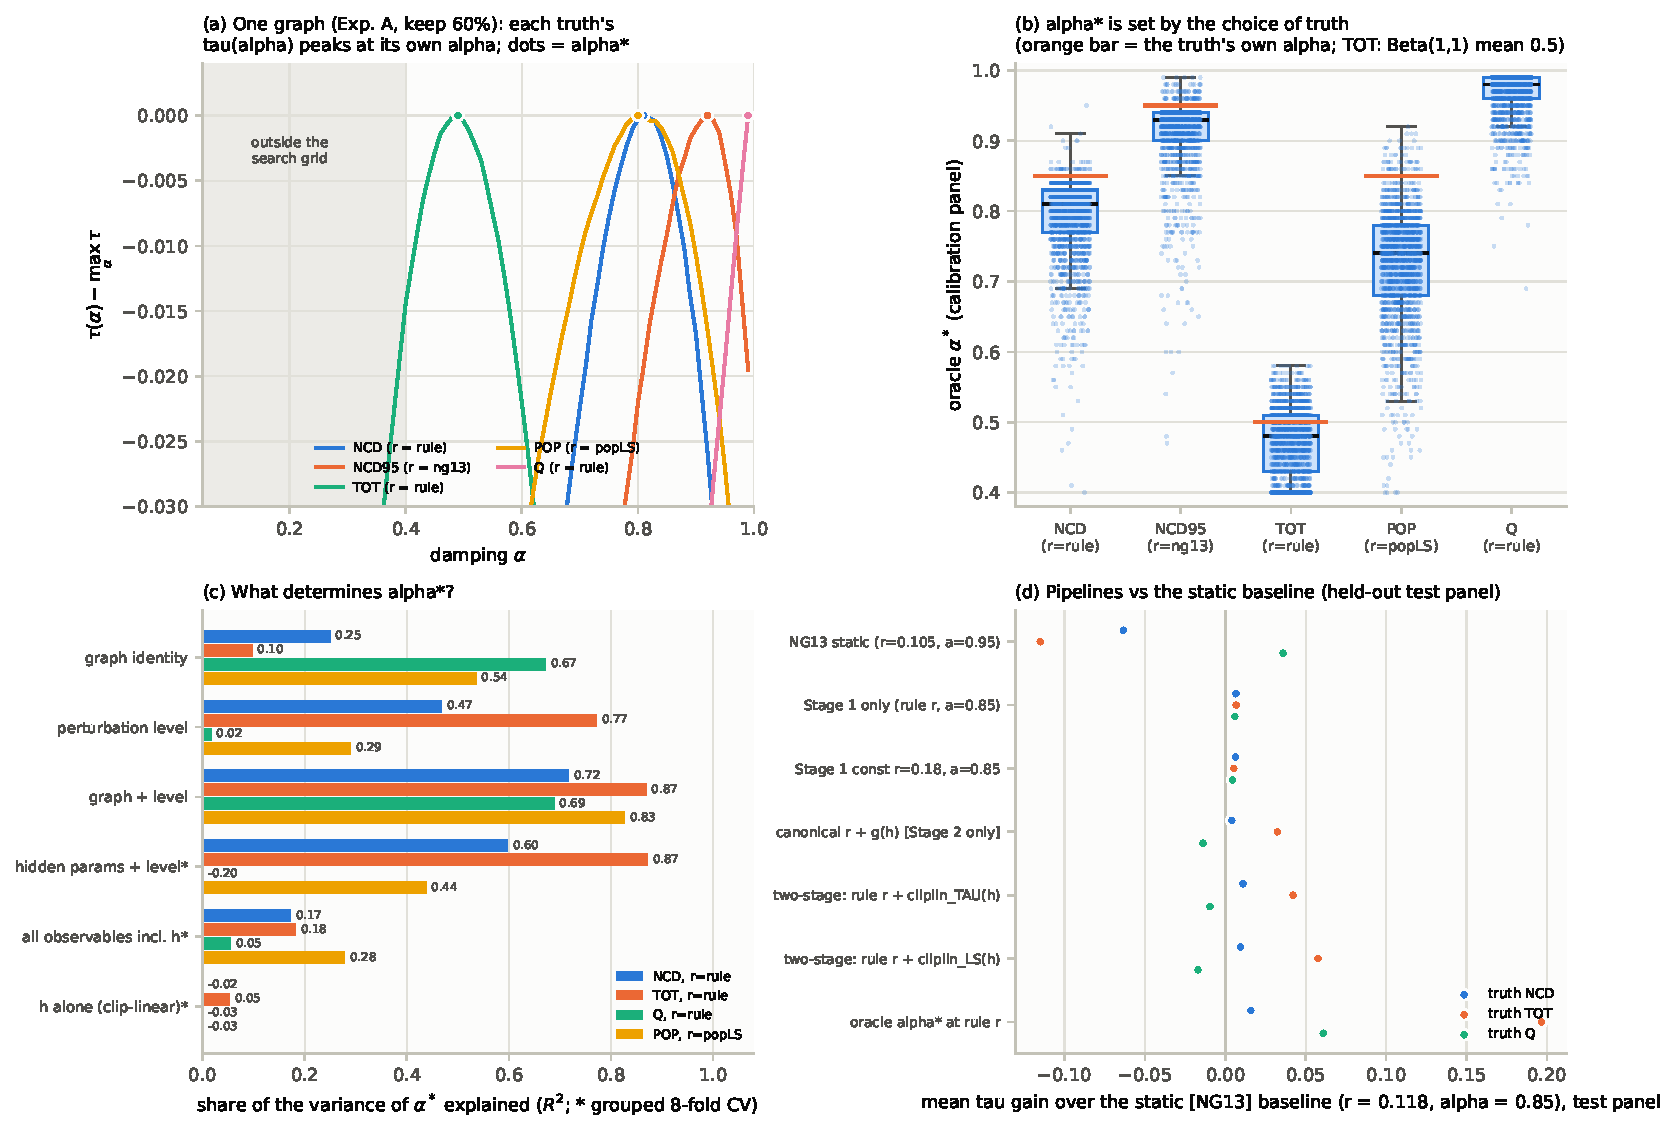
\includegraphics[width=\textwidth]{stage2_diagnostics.pdf}
\caption{Stage~2 diagnostics. \textbf{(a)} For one calibration graph (Experiment~A, $60\%$ of arcs kept),
the curve $\tau(\alpha)-\max\tau$ under each truth peaks near the damping that defines that truth.
\textbf{(b)} Distribution of $\alpha^*$ per truth; orange bars mark each truth's own $\alpha$.
\textbf{(c)} Share of the variance of $\alpha^*$ explained. \textbf{(d)} Gain over the static setting
$(0.118,0.85)$ on \texttt{test} for complete pipelines under three truths. The sign of the two-stage
gain flips between truths.}
\label{fig:s2diag}
\end{figure}

\begin{figure}[t]
\centering
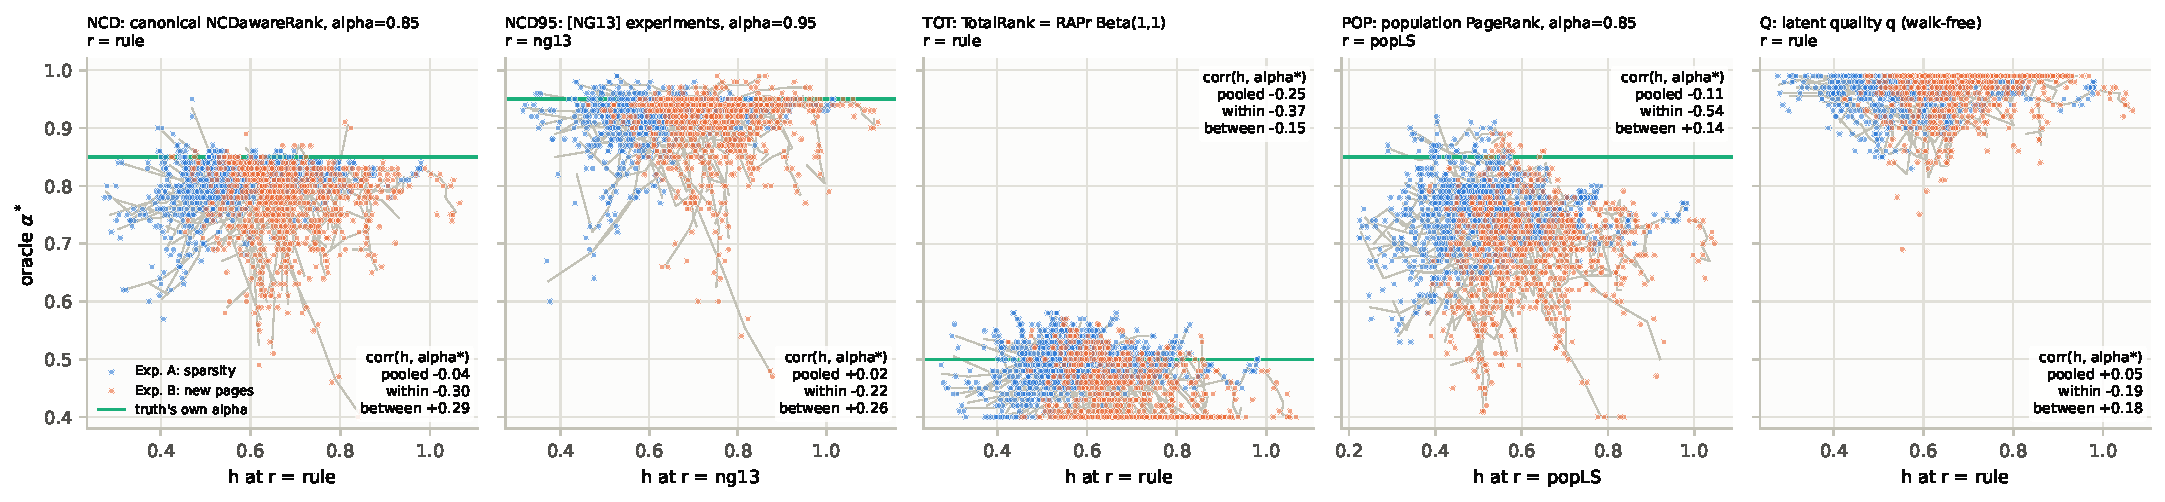
\includegraphics[width=\textwidth]{stage2_gt_sensitivity.pdf}
\caption{Oracle damping against $h$ under the five truths (calibration panel). Within each truth the
relation with $h$ is weak and of mixed sign; across truths the level of $\alpha^*$ follows the damping
that defines the truth (green line).}
\label{fig:s2truth}
\end{figure}

\subsection{Complete pipelines against the static settings}
Table~\ref{tab:pipe} compares complete $(r,\alpha)$ pipelines with the two published static settings,
under all five truths and on all panels. Under the primary truth, the two-stage pipeline (locked rule
for $r$, $\alpha=\STwoConstAlpha$) improves on the canonical setting $(0.118,0.85)$ by \TwoTestD{} on
\texttt{test} (95\% CI $[\TwoTestLo,\TwoTestHi]$, better on \TwoTestWins{} graphs, $p=\TwoTestP$),
\TwoScaleD{} on \texttt{scale} (\TwoScaleWins) and \TwoTopoD{} on \texttt{topo} (\TwoTopoWins). This is
about two thirds of the oracle headroom on \texttt{test} (\PipeNcdOracleVsLoTest). The gain splits into
\StoTestD{} from Stage~1 ($p=\StoTestP$) and \SthTestD{} from Stage~2 ($p=\SthTestP$). On \texttt{real}
it is \TwoRealD{} per graph (95\% CI $[\TwoRealLo,\TwoRealHi]$, \TwoRealWins{} graphs, $p=\TwoRealP$):
\TwoRealCnr{} on cnr-2000, \TwoRealCorafull{} on Cora, \TwoRealCiteseer{} on CiteSeer, \TwoRealCoraml{}
on Cora-ML and \TwoRealWikics{} on WikiCS (Appendix Table~\ref{tab:realdetail}).

The verdict depends on the truth (Figure~\ref{fig:s2diag}d). The same locked pipeline:
\begin{itemize}[leftmargin=1.4em,itemsep=0pt]
\item beats the canonical setting under TOT (\PipeTotTwoVsLoTest) and POP (\PipePopTwoVsLoTest), simply
because $0.81$ is closer than $0.85$ to those truths' anchors;
\item loses to the setting $(0.105,0.95)$ of~\cite{ng13} under NCD95 (\PipeNcdnfTwoVsHiTest) and under
the walk-free Q (\PipeQTwoVsHiTest), whose anchors lie above $0.9$.
\end{itemize}
Claims that a calibrated damping ``beats the default'' are therefore claims about the reference as much
as about the method.

\begin{table*}[t]
\centering
\scriptsize
\caption{Complete pipelines against the static [NG13] settings under all five truths. Cells: mean Kendall $\tau$ over instances; in parentheses, the difference against [NG13] $(0.118,0.85)$ averaged over graphs (each graph weighted equally). \emph{Two-stage}: $r$ from the locked Stage~1 rule and $\alpha=0.81$, both fitted on calibration graphs under NCD and applied unchanged under every truth. POP and Q exist only for the static generator.}
\label{tab:pipe}
\begin{tabular}{@{}lccccc@{}}
\toprule
policy $(r,\alpha)$ & \texttt{calib} & \texttt{test} & \texttt{scale} & \texttt{topo} & \texttt{real} \\
\midrule
\multicolumn{6}{@{}l}{\textit{truth NCD}} \\
\quad [NG13] $(0.118,\,0.85)$ & 0.6805 & 0.6801 & 0.6633 & 0.7840 & 0.7559 \\
\quad [NG13] $(0.105,\,0.95)$ & 0.6133 ($-$0.0673) & 0.6168 ($-$0.0633) & 0.5979 ($-$0.0654) & 0.7360 ($-$0.0479) & 0.6792 ($-$0.0831) \\
\quad Stage 1 only & 0.6862 ($+$0.0056) & 0.6867 ($+$0.0066) & 0.6681 ($+$0.0049) & 0.7844 ($+$0.0005) & 0.7600 ($+$0.0030) \\
\quad two-stage ($\alpha=0.81$) & 0.6913 ($+$0.0108) & 0.6911 ($+$0.0110) & 0.6735 ($+$0.0102) & 0.7875 ($+$0.0036) & 0.7559 ($+$0.0017) \\
\quad oracle $\alpha^*$ & 0.6965 ($+$0.0160) & 0.6960 ($+$0.0159) & 0.6787 ($+$0.0155) & 0.7911 ($+$0.0071) & 0.7738 ($+$0.0189) \\
\multicolumn{6}{@{}l}{\textit{truth NCD95}} \\
\quad [NG13] $(0.118,\,0.85)$ & 0.6227 & 0.6237 & 0.6044 & 0.7472 & 0.6678 \\
\quad [NG13] $(0.105,\,0.95)$ & 0.6410 ($+$0.0182) & 0.6431 ($+$0.0194) & 0.6226 ($+$0.0183) & 0.7576 ($+$0.0104) & 0.7122 ($+$0.0449) \\
\quad Stage 1 only & 0.6282 ($+$0.0055) & 0.6306 ($+$0.0069) & 0.6096 ($+$0.0052) & 0.7472 ($-$0.0001) & 0.6767 ($+$0.0104) \\
\quad two-stage ($\alpha=0.81$) & 0.6103 ($-$0.0125) & 0.6128 ($-$0.0109) & 0.5920 ($-$0.0124) & 0.7404 ($-$0.0069) & 0.6463 ($-$0.0206) \\
\quad oracle $\alpha^*$ & 0.6530 ($+$0.0303) & 0.6560 ($+$0.0323) & 0.6343 ($+$0.0299) & 0.7660 ($+$0.0188) & 0.7281 ($+$0.0609) \\
\multicolumn{6}{@{}l}{\textit{truth TOT}} \\
\quad [NG13] $(0.118,\,0.85)$ & 0.5893 & 0.5932 & 0.5773 & 0.7624 & 0.6804 \\
\quad [NG13] $(0.105,\,0.95)$ & 0.4689 ($-$0.1204) & 0.4782 ($-$0.1150) & 0.4591 ($-$0.1183) & 0.7001 ($-$0.0623) & 0.5387 ($-$0.1461) \\
\quad Stage 1 only & 0.5963 ($+$0.0071) & 0.6000 ($+$0.0068) & 0.5854 ($+$0.0080) & 0.7655 ($+$0.0030) & 0.6688 ($-$0.0128) \\
\quad two-stage ($\alpha=0.81$) & 0.6341 ($+$0.0449) & 0.6354 ($+$0.0422) & 0.6230 ($+$0.0457) & 0.7775 ($+$0.0151) & 0.7097 ($+$0.0298) \\
\quad oracle $\alpha^*$ & 0.7987 ($+$0.2094) & 0.7899 ($+$0.1967) & 0.7839 ($+$0.2065) & 0.8094 ($+$0.0469) & 0.8336 ($+$0.1582) \\
\multicolumn{6}{@{}l}{\textit{truth POP}} \\
\quad [NG13] $(0.118,\,0.85)$ & 0.5462 & 0.5446 & 0.5172 & -- & -- \\
\quad [NG13] $(0.105,\,0.95)$ & 0.4904 ($-$0.0558) & 0.4957 ($-$0.0490) & 0.4683 ($-$0.0489) & -- & -- \\
\quad Stage 1 only & 0.5510 ($+$0.0048) & 0.5506 ($+$0.0060) & 0.5237 ($+$0.0065) & -- & -- \\
\quad two-stage ($\alpha=0.81$) & 0.5614 ($+$0.0152) & 0.5585 ($+$0.0139) & 0.5326 ($+$0.0154) & -- & -- \\
\quad oracle $\alpha^*$ & 0.5745 ($+$0.0283) & 0.5677 ($+$0.0231) & 0.5443 ($+$0.0271) & -- & -- \\
\multicolumn{6}{@{}l}{\textit{truth Q}} \\
\quad [NG13] $(0.118,\,0.85)$ & 0.3655 & 0.3478 & 0.3302 & -- & -- \\
\quad [NG13] $(0.105,\,0.95)$ & 0.3939 ($+$0.0283) & 0.3837 ($+$0.0359) & 0.3560 ($+$0.0258) & -- & -- \\
\quad Stage 1 only & 0.3724 ($+$0.0069) & 0.3537 ($+$0.0059) & 0.3332 ($+$0.0030) & -- & -- \\
\quad two-stage ($\alpha=0.81$) & 0.3585 ($-$0.0070) & 0.3382 ($-$0.0096) & 0.3202 ($-$0.0100) & -- & -- \\
\quad oracle $\alpha^*$ & 0.4150 ($+$0.0495) & 0.4087 ($+$0.0609) & 0.3712 ($+$0.0410) & -- & -- \\
\bottomrule
\end{tabular}
\end{table*}


\subsection{Convergence}
Lowering $\alpha$ also shortens the power iteration. This holds for any lower $\alpha$ and is a side
benefit, not a property of the calibration. The a-priori estimate $k\approx\ln\varepsilon/\ln\alpha$,
based on $|\lambda_2(P)|\le\alpha$~\cite{haveliwala03,ng13}, predicts savings of \ConvNcdBound\% for
$0.85\to0.81$ ($\ConvNcdBoundK$ iterations at $\varepsilon=10^{-6}$) and \ConvNfBound\% for
$0.95\to0.93$. The measured savings are smaller. The actual contraction is faster than $\alpha$, so
both iteration counts stay well below the estimate (Table~\ref{tab:conv}), and the saving is
\ConvNcdTest\% on \texttt{test} and \ConvNcdReal\% on \texttt{real} for the NCD branch, and \ConvNfTest\%
and \ConvNfReal\% for the NCD95 branch.

\begin{table*}[t]
\centering
\small
\caption{Power-iteration counts before and after the noise discount (stopping rule $\|\pi^{(k+1)}-\pi^{(k)}\|_1<\varepsilon=10^{-6}$, start $v$). The bound column is the a-priori estimate from $|\lambda_2(P)|\le\alpha$; measured columns are mean counts over all perturbed instances of the panel.}
\label{tab:conv}
\begin{tabular}{@{}lllll@{}}
\toprule
configuration & $\alpha$ & bound $\ln\varepsilon/\ln\alpha$ & measured, \texttt{test} & measured, \texttt{real} \\
\midrule
NCD branch ($r$ = rule) & 0.85$\to$0.81 & 85$\to$66 ($-22.9\%$) & 30.2$\to$25.8 ($-14.7\%$) & 30.5$\to$26.5 ($-13.1\%$) \\
NCD95 branch ($r=0.105$) & 0.95$\to$0.93 & 269$\to$190 ($-29.3\%$) & 67.2$\to$54.2 ($-19.3\%$) & 69.9$\to$59.2 ($-15.3\%$) \\
\bottomrule
\end{tabular}
\end{table*}


\subsection{Sensitivity truths with refitted rules}
Refitting $g$ separately for each truth does not change the conclusion (Appendix
Table~\ref{tab:sens}). Under Q, POP and NCD95, the $\tau$-optimised rule on $h$ is the constant or
indistinguishable from it. Under TOT, $h$ carries a weak signal with the same negative sign within and
between graphs. It gains \TotHTest{} on \texttt{test} ($p=\TotHTestP$), but \TotHTopo{} on \texttt{topo}
and \TotHReal{} on \texttt{real}, so it does not transfer.

\FloatBarrier
% =============================================================================
\section{Discussion}
\label{sec:discussion}

\paragraph{What the calibration achieves.} Against the canonical reference, the two-stage procedure
amounts to re-tuning two constants: more weight on the proximity matrix ($r\approx0.2$, $\mu\approx0.17$
instead of $0.10$) and slightly less damping ($\alpha=\STwoConstAlpha$ instead of $0.85$). On held-out
synthetic graphs, including larger graphs and a different generative mechanism, the gain is
$0.004$--$0.011$ in Kendall's $\tau$, consistent across graphs, plus a modest acceleration. On five real networks
the gain is not distinguishable from zero. These are honest, if modest, results for a zero-cost
procedure. They are not the adaptive, structure-driven calibration that motivated the study.

\paragraph{Why structural statistics fail here.} The oracle parameters depend on two quantities: how
severely the observed graph is perturbed relative to the reference, and the latent quality structure
of the pages. Neither is revealed by global statistics of the observed graph. $\Pbar$ and $h$ react
strongly to link loss inside a graph. Across graphs their levels are confounded with ordinary
structural variation, and $h$ responds to different kinds of link loss with opposite signs.
Section~\ref{sec:hmech} isolates the missing ingredient: given the unperturbed graph's own value $h_0$,
a tent in $h-h_0$ recovers \NmDhShare\% of the oracle headroom in cross-validation, whereas none of
\NmRules{} rules on statistics of the observed graph alone passes the held-out test. The statistic
could therefore become useful where a less perturbed snapshot of the same graph is available as a
reference; we have not tested this. A related
pattern appeared in our earlier work on uncertain graphs~\cite{konstantellos26}: there, the correlation
between the escape probability and the optimal damping did not survive on real networks, and routing
among heuristics by the same statistic worked on synthetic graphs but failed on real ones. We take this
as evidence that single global statistics are too coarse to transfer parameter choices between graphs.

\paragraph{Anchoring as a methodological lesson.} The strongest finding is not about NCDawareRank. When a
ranking method is tuned to agree with a reference ranking, the optimal damping is the reference's own
damping minus a noise discount. This follows from the dose-response test and from five truths with
very different anchors. Any statement that one damping factor is ``better'' therefore inherits the
damping of the ground truth. The two $\alpha$-free references available to us disagree by almost
$0.5$, which suggests that no truth-independent optimal damping exists for this problem. Evaluations
of damping choices should report results under several references, and stability protocols should not
be used to choose parameters.

\paragraph{What the theory of $h$ offers.} The identities of Proposition~\ref{prop:interp} and the bound
of Theorem~\ref{thm:bound} give $h$ and $h_v$ a precise meaning: they measure how strongly the chain
pushes rank away from the uniform and the teleportation distribution, and $h_v$ bounds the total
displacement of the ranking for every $\alpha$. They are useful diagnostics, for example for deciding
whether the damping matters at all for a given graph. The empirical results show that they are not
calibration statistics.

\paragraph{Limitations.} The synthetic generators, however varied, are our own. The partition of
cnr-2000 is a host proxy and the citation graphs use topic labels, not hosts. Dangling pages are handled
by uniform rows, not by the block-confined strategy of~\cite{ng20}. Stage~1 is anchored at
$\alpha_0=0.85$, and the Stage~2 grid stops at $0.99$, which censors the oracle under Q (we checked that
the optimum does not lie beyond it). We evaluate rank correlations only, against references derived from
models. External relevance judgements or browsing data, as in~\cite{gleich10}, would provide a ground
truth that does not depend on a damping factor.

% =============================================================================
\section{Conclusion}
\label{sec:conclusion}

We formulated a two-stage, zero-cost calibration of NCDawareRank. The mixing ratio comes from the block
escape probability and the total damping from the deviation of the ensembled operator from double
stochasticity. We proved identities and a displacement bound that give these statistics a precise
meaning. A large, cluster-aware evaluation shows that the statistics do not predict the optimal
parameters. The calibration reduces to two constants, $r\approx0.2$ and $\alpha=\STwoConstAlpha$, that
improve the recovery of the canonical ranking on synthetic graphs by $0.004$--$0.011$ in Kendall's $\tau$
and leave real networks unchanged. The optimal damping is anchored to the damping of the reference ranking,
minus a noise discount. The choice of ground truth therefore decides which parameter setting wins, and
we recommend that future comparisons of link-analysis parameters report results under several
references.

\section*{Reproducibility}
All code, raw results and figures accompany the paper; the accompanying documentation describes every
module. In brief:
\begin{itemize}[leftmargin=1.4em,itemsep=0pt]
\item \texttt{prepare\_real\_graphs.py} builds the real panel;
\item \texttt{run\_experiments.py stage1} and \texttt{run\_experiments.py stage2} run both stages;
\item \texttt{stage1\_analysis.py}, \texttt{stage2\_analysis.py} and the decomposition, anchoring,
convergence and bound-check scripts produce every number;
\item \texttt{make\_paper\_assets.py} writes the numbers and tables of this manuscript directly from the
result files.
\end{itemize}
Unit tests check the implementation against the matrices of~\cite[Fig.~1]{ng13}, Theorems~1--2
of~\cite{ng13}, dense solves, quadrature and the bound~\eqref{eq:bound}.

% =============================================================================
\begin{thebibliography}{PBMW99}
\raggedright
\small
\bibitem[ALP08]{avrachenkov08} K.~Avrachenkov, N.~Litvak, K.~S.~Pham. A singular perturbation approach for
choosing the PageRank damping factor. \emph{Internet Mathematics}, 5(1--2):47--69, 2008.
\bibitem[BBC06]{baeza06} R.~Baeza-Yates, P.~Boldi, C.~Castillo. Generic damping functions for propagating
importance in link-based ranking. \emph{Internet Mathematics}, 3(4):445--478, 2006.
\bibitem[BCSV04]{boldi04ubi} P.~Boldi, B.~Codenotti, M.~Santini, S.~Vigna. UbiCrawler: a scalable fully
distributed Web crawler. \emph{Software: Practice and Experience}, 34(8):711--726, 2004.
\bibitem[BG18]{bojchevski18} A.~Bojchevski, S.~G\"unnemann. Deep Gaussian embedding of graphs: unsupervised
inductive learning via ranking. In \emph{Proc.\ ICLR}, 2018.
\bibitem[BNG19]{berberidis19} D.~Berberidis, A.~N.~Nikolakopoulos, G.~B.~Giannakis. Adaptive diffusions for
scalable learning over graphs. \emph{IEEE Trans.\ Signal Processing}, 67(5):1307--1321, 2019.
\bibitem[Bol05]{boldi05tr} P.~Boldi. TotalRank: ranking without damping. In \emph{Special Interest Tracks and
Posters of the 14th WWW}, 898--899, 2005.
\bibitem[BP10]{bressan10} M.~Bressan, E.~Peserico. Choose the damping, choose the ranking? \emph{J.\ Discrete
Algorithms}, 8(2):199--213, 2010.
\bibitem[BSV05]{boldi05} P.~Boldi, M.~Santini, S.~Vigna. PageRank as a function of the damping factor. In
\emph{Proc.\ 14th WWW}, 557--566, 2005.
\bibitem[BSV09]{boldi09} P.~Boldi, M.~Santini, S.~Vigna. PageRank: functional dependencies. \emph{ACM Trans.\
Information Systems}, 27(4):19, 2009.
\bibitem[BV04]{boldi04} P.~Boldi, S.~Vigna. The WebGraph framework I: compression techniques. In \emph{Proc.\
13th WWW}, 595--602, 2004.
\bibitem[CG09]{constantine09} P.~G.~Constantine, D.~F.~Gleich. Random alpha PageRank. \emph{Internet
Mathematics}, 6(2):189--236, 2009.
\bibitem[Cou77]{courtois77} P.-J.~Courtois. \emph{Decomposability: Queueing and Computer System Applications}.
Academic Press, 1977.
\bibitem[ET93]{efron93} B.~Efron, R.~J.~Tibshirani. \emph{An Introduction to the Bootstrap}. Chapman \& Hall,
1993.
\bibitem[FBFM08]{fortunato08} S.~Fortunato, M.~Bogu\~n\'a, A.~Flammini, F.~Menczer. Approximating PageRank from
in-degree. In \emph{Algorithms and Models for the Web-Graph (WAW 2006)}, LNCS 4936, 59--71, 2008.
\bibitem[Fri01]{friedman01} J.~H.~Friedman. Greedy function approximation: a gradient boosting machine.
\emph{Annals of Statistics}, 29(5):1189--1232, 2001.
\bibitem[GCFG10]{gleich10} D.~F.~Gleich, P.~G.~Constantine, A.~D.~Flaxman, A.~Gunawardana. Tracking the random
surfer: empirically measured teleportation parameters in PageRank. In \emph{Proc.\ 19th WWW}, 381--390,
2010.
\bibitem[HK03]{haveliwala03} T.~H.~Haveliwala, S.~D.~Kamvar. The second eigenvalue of the Google matrix.
Technical Report 2003-20, Stanford InfoLab, 2003.
\bibitem[Ken38]{kendall38} M.~G.~Kendall. A new measure of rank correlation. \emph{Biometrika}, 30(1/2):81--93,
1938.
\bibitem[Ken45]{kendall45} M.~G.~Kendall. The treatment of ties in ranking problems. \emph{Biometrika},
33(3):239--251, 1945.
\bibitem[KH03]{kamvar03} S.~D.~Kamvar, T.~H.~Haveliwala. The condition number of the PageRank problem.
Technical Report 2003-36, Stanford InfoLab, 2003.
\bibitem[Kon26]{konstantellos26} I.~Konstantellos. Damping from the escape probability: a free calibration
rule for diffusion-based reachability ranking in uncertain graphs. Computer Engineering and Informatics
Department, University of Patras, 2026. Zenodo record \url{https://zenodo.org/records/23211440}.
\bibitem[LM06]{langville06} A.~N.~Langville, C.~D.~Meyer. \emph{Google's PageRank and Beyond: The Science of
Search Engine Rankings}. Princeton University Press, 2006.
\bibitem[LSV07]{litvak07} N.~Litvak, W.~R.~W.~Scheinhardt, Y.~Volkovich. In-degree and PageRank: why do they
follow similar power laws? \emph{Internet Mathematics}, 4(2--3):175--198, 2007.
\bibitem[MC20]{mernyei20} P.~Mernyei, C.~Cangea. Wiki-CS: a Wikipedia-based benchmark for graph neural
networks. arXiv:2007.02901, 2020.
\bibitem[NG13]{ng13} A.~N.~Nikolakopoulos, J.~D.~Garofalakis. NCDawareRank: a novel ranking method that
exploits the decomposable structure of the Web. In \emph{Proc.\ 6th ACM WSDM}, 143--152, 2013.
\bibitem[Nik20]{ng20} A.~N.~Nikolakopoulos. Random surfing revisited: generalizing PageRank's teleportation
model. arXiv:2008.12916, 2020.
\bibitem[PBMW99]{page99} L.~Page, S.~Brin, R.~Motwani, T.~Winograd. The PageRank citation ranking: bringing order
to the Web. Technical Report 1999-66, Stanford InfoLab, 1999.
\bibitem[SA61]{simon61} H.~A.~Simon, A.~Ando. Aggregation of variables in dynamic systems. \emph{Econometrica},
29(2):111--138, 1961.
\bibitem[Wil45]{wilcoxon45} F.~Wilcoxon. Individual comparisons by ranking methods. \emph{Biometrics Bulletin},
1(6):80--83, 1945.
\end{thebibliography}

% =============================================================================
\FloatBarrier
\appendix
\section{Additional tables}
\label{app:tables}
Table~\ref{tab:stage1truth} repeats the Stage~1 comparison under the four Stage~1 truths.
Table~\ref{tab:sens} refits the Stage~2 rule separately for each sensitivity truth.
Table~\ref{tab:realdetail} breaks the real panel down by network.

\begin{table}[!htbp]
\centering
\footnotesize\setlength{\tabcolsep}{4pt}
\caption{Stage~1 under the four Stage~1 truths. Const $r$: the best constant on the calibration panel; $\tau$-opt.\ rule: the $\tau$-optimised clip-linear rule on $\bar P=\bar P^{(M)}_{\mathrm{esc}}$. Canonical $\tau$: mean Kendall $\tau$ of the canonical $r=0.118$ on \texttt{test}; const $-$ can.: gain of the constant over it. The last four columns give the mean $\tau$ difference between the rule and the constant per panel. $^{\dagger}$: Wilcoxon signed-rank $p<0.01$ over graphs. POP exists only for the static generator. Under SELF both the constant and the rule sit at the upper bound $r=0.99$.}
\label{tab:stage1truth}
\begin{tabular}{@{}lllrrrrrr@{}}
\toprule
& & & \multicolumn{2}{c}{\texttt{test}} & \multicolumn{4}{c}{rule $-$ constant} \\
\cmidrule(lr){4-5}\cmidrule(l){6-9}
truth & const $r$ & $\tau$-opt.\ rule & canonical $\tau$ & const $-$ can. & \texttt{test} & \texttt{scale} & \texttt{topo} & \texttt{real} \\
\midrule
NCD & $0.18$ & $\mathrm{clip}(0.242-0.143\,\bar P)$ & 0.6801 & $+$0.0063$^{\dagger}$ & $+$0.0003 & 0.0000 & $+$0.0007 & $+$0.0008 \\
PR & $0.02$ & $\mathrm{clip}(-0.017-0.075\,\bar P)$ & 0.6569 & $+$0.0083 & $-$0.0002 & 0.0000 & $+$0.0016$^{\dagger}$ & $+$0.0015 \\
POP & $0.23$ & $\mathrm{clip}(0.448-0.547\,\bar P)$ & 0.5446 & $+$0.0067$^{\dagger}$ & $+$0.0006 & $+$0.0016 & -- & -- \\
SELF & $0.99$ & $\mathrm{clip}(0.960+0.836\,\bar P)$ & 0.6801 & $+$0.1504$^{\dagger}$ & 0.0000 & 0.0000 & 0.0000 & $+$0.0040 \\
\bottomrule
\end{tabular}
\end{table}

\begin{table}[!htbp]
\centering
\footnotesize\setlength{\tabcolsep}{4pt}
\caption{Sensitivity truths, with $g$ refitted for each truth: mean $\tau$ difference of the $\tau$-optimised clip-linear rule on $h$ against the truth's best constant $\alpha$ (Wilcoxon $p$ over graphs). A dash means the panel has no such truth, or the rule equals the constant.}
\label{tab:sens}
\begin{tabular}{@{}lllllll@{}}
\toprule
truth & const $\alpha$ & $\tau$-optimised $g(h)$ & \texttt{test} & \texttt{scale} & \texttt{topo} & \texttt{real} \\
\midrule
TOT & $0.48$ & $\mathrm{clip}(0.561-0.129\,h)$ & $+$0.0006 (0.002) & $+$0.0002 (0.569) & $-$0.0001 (0.053) & $-$0.0020 (0.062) \\
Q & $0.99$ & $\mathrm{clip}(0.939+0.093\,h)$ & $-$0.0011 (0.008) & $-$0.0006 (0.359) & -- & -- \\
POP ($r$: LS rule) & $0.74$ & $\mathrm{clip}(0.779-0.075\,h)$ & $+$0.0003 (0.062) & $-$0.0002 (0.339) & -- & -- \\
POP ($r$: $\tau$-opt.\ rule) & $0.74$ & $\mathrm{clip}(0.761-0.041\,h)$ & $+$0.0001 (0.098) & $-$0.0001 (0.339) & -- & -- \\
NCD95 & $0.93$ & $\mathrm{clip}(0.930-0.000\,h)$ & 0.0000 (--) & 0.0000 (--) & 0.0000 (--) & 0.0000 (--) \\
\bottomrule
\end{tabular}
\end{table}

\begin{table}[!htbp]
\centering
\footnotesize
\caption{Real networks, truth NCD: mean Kendall $\tau$ per graph over the perturbed instances, and the mean oracle damping under NCD and TOT.}
\label{tab:realdetail}
\begin{tabular}{@{}lrrrrrrr@{}}
\toprule
graph & mean $r$ & [NG13] $(0.118,0.85)$ & Stage 1 & two-stage & oracle & $\alpha^*$ NCD & $\alpha^*$ TOT \\
\midrule
cnr-2000 & 0.230 & 0.7505 & 0.7435 & 0.7678 & 0.7788 & 0.772 & 0.521 \\
WikiCS & 0.181 & 0.7927 & 0.7933 & 0.7878 & 0.7956 & 0.835 & 0.508 \\
Cora (full) & 0.207 & 0.7513 & 0.7461 & 0.7533 & 0.7550 & 0.811 & 0.474 \\
Cora-ML & 0.225 & 0.7452 & 0.7392 & 0.7420 & 0.7471 & 0.831 & 0.480 \\
CiteSeer & 0.240 & 0.7370 & 0.7696 & 0.7346 & 0.7949 & 0.850 & 0.510 \\
\bottomrule
\end{tabular}
\end{table}


\end{document}
